\input{|"./setup.sh"}
% !TEX root = ../Robotik.tex
\documentclass[a4paper, fontsize=12pt, ngerman, oneside, openright]{scrreprt}

% Rendering packages
\usepackage{amsmath}
\usepackage{amssymb}
%\usepackage[draft]{graphicx}
\usepackage{graphicx}
\usepackage{wrapfig}
\usepackage{svg}
\usepackage{subcaption}
\usepackage{placeins}
\usepackage{xcolor}      % use if color is used in text
\usepackage{eurosym}
\usepackage{float}
\usepackage[toc,page]{appendix}

% Page dimensions
\usepackage[inner=2.0cm,outer=2.0cm,top=1.7cm,bottom=1.9cm]{geometry}
\usepackage{parskip}
\usepackage[onehalfspacing]{setspace}

% Font styling
\usepackage[english]{babel}
\usepackage[utf8]{inputenc}
\usepackage[T1]{fontenc}
\usepackage{lmodern}
\renewcommand\familydefault{\sfdefault}
\usepackage[11pt]{moresize}

% Tables
\usepackage{tabularx}
\usepackage{tabulary}
\usepackage{longtable, lscape}

% Headers
\usepackage{scrpage2}  % header and footer for KOMA-Script
\pagestyle{scrheadings}
\automark[section]{chapter}

% Zitate
\usepackage[backend=biber,
			style=authoryear,
			isbn=false,
			sorting=nyt,
			]{biblatex}
\usepackage[babel,german=quotes, english=british, threshold=3]{csquotes}
\bibliography{Bibliothek/Bibliothek}

\usepackage[hyperindex,breaklinks,colorlinks=true,linkcolor=black,urlcolor=blue,citecolor=black]{hyperref}

% Code Blöcke
\usepackage{listings}
%\usepackage{Header/listings-golang} % import this package after listings
\usepackage{syntax}



%\lstset{ % add your own preferences
%	frame=single,
%	captionpos=b,
%	mathescape=true,
%	basicstyle=\footnotesize\ttfamily,
%	keywordstyle=\color{black},
%	numbers=left,
%	numbersep=5pt,
%	showstringspaces=false,
%	stringstyle=\color{blue},
%	tabsize=2,
%	language=Golang % this is it !
%}


%table colors
\usepackage{xcolor,colortbl}

\newcommand{\mc}[2]{\multicolumn{#1}{c}{#2}}
\definecolor{Gray}{gray}{0.85}
\definecolor{LightCyan}{rgb}{0.88,1,1}

\newcolumntype{a}{>{\columncolor{Gray}}c}
\newcolumntype{b}{>{\columncolor{Gray}}l}

\usepackage{color}
\definecolor{gray}{rgb}{0.4,0.4,0.4}
\definecolor{darkblue}{rgb}{0.0,0.0,0.6}
\definecolor{cyan}{rgb}{0.0,0.6,0.6}
\definecolor{dkgreen}{rgb}{0,0.6,0}
\definecolor{gray}{rgb}{0.5,0.5,0.5}
\definecolor{mauve}{rgb}{0.58,0,0.82}

\lstset{
  basicstyle=\ttfamily,
  columns=fullflexible,
  showstringspaces=false,
  commentstyle=\color{gray}\upshape
}

\lstset{
	frame=tb,
	language=Java,
	aboveskip=3mm,
	belowskip=3mm,
	showstringspaces=false,
	columns=flexible,
	basicstyle={\small\ttfamily},
	numbers=none,
	numberstyle=\tiny\color{gray},
	keywordstyle=\color{blue},
	commentstyle=\color{dkgreen},
	stringstyle=\color{mauve},
	breaklines=true,
	breakatwhitespace=true,
	tabsize=4,
	numbers=left
}

\lstdefinelanguage{XML}
{
	morestring=[b]",
	morestring=[s]{>}{<},
	morecomment=[s]{<?}{?>},
	morecomment=[s]{!--}{--},
	stringstyle=\color{black},
	identifierstyle=\color{darkblue},
	keywordstyle=\color{cyan} list your attributes here
}

%pdf insert
\usepackage{pdfpages}

%zusätzliche Trennungen
\hyphenation{Grund-ar-chi-tek-tur}
\hyphenation{MQTT-Kom-mu-ni-ka-tions-mo-dell}
\hyphenation{Master-Master-Replikation}
\hyphenation{Pub-lish-er}
\hyphenation{Pub-lish-ers}
\hyphenation{Sub-scriber}
\hyphenation{Sub-scribers}
\hyphenation{Pub-lish er/Sub-scriber}
\hyphenation{beo-bacht-bar}
\hyphenation{Score}
\hyphenation{Ac-knowl-edge-ment}
\hyphenation{Ac-knowl-edge-ments}

\usepackage{mathtools}
\DeclarePairedDelimiter\abs{\lvert}{\rvert}

\usepackage{acronym}
\setstretch{1.0}

\newcommand\tab[1][1cm]{\hspace*{#1}}

\begin{document}

% Titelseite einfügen.
%% !TEX root = ../Robotik.tex
\begin{titlepage}


\begin{center}
 		\includegraphics[scale=1]{Resources/Haw}
\end{center}

\begin{center}
	\HUGE \textbf{Robotik Zusammenfassung}
	\large\\Prof. Schiedermeier\\ \ \\

	SS 2019
\end{center}

\begin{center}
Robin Atherton
\end{center}

\end{titlepage}

\clearpage

% Counter zurücksetzen. Römische Ziffern einstellen.
\pagenumbering{Roman}
\setcounter{page}{1}

% Inhaltsverzeichnis generieren.
\tableofcontents

% Neue Seite. Counter zurücksetzen. Arabische Ziffern einstellen.
\clearpage
\pagenumbering{arabic}
\setcounter{page}{1}

% Kapitel einfügen.
% !TEX root = ../Robotik.tex
\chapter{Geschichte}
\section{Industrieroboter}
Nach Definition der VDI-Richtlinie 2860 sind Industrieroboter universell einsetzbare Bewegungsautomaten mit meherern Achsen, deren Bewegungen hinsichtlich Bewegungsfolge und Wegen bzw. Winkel frei programmierbar und sensorgeführt sind.
\begin{itemize}
	\item Zeichnen sich durch \textbf{Schnelligkeit}, \textbf{Genauigkeit}, \textbf{Robustheit }und eine hohe \textbf{Traglast }aus.
	\item Einsatzgebiete: Schweißen, Kleben, Schneide, Lackieren
\end{itemize}
Zunehmend \textbf{kollaborative} Roboter, Cobots:
\begin{itemize}
	\item Industrieroboter, die mit Menschen gemeinsam arbeiten
	\item Nicht mehr durch Schutzeinrichtungen im Produktionsprozess von Menschen getrennt
	\item Nimmt Menschen wahr, verursacht keine Verletzungen
\end{itemize}

\section{Serviceroboter}
\subsection{Definition}
\begin{itemize}
	\item Ein \textbf{Serviceroboter} ist eine \textbf{frei programmierbare Bewegungseinrichtung}, die \textbf{teil- oder vollautomatisch} Dienstleistungen verrichtet.
	\item \textbf{Dienstleistungen} sind dabei Tätigkeiten, die nicht der direkten industriellen ERzeugung von Sachgütern, sondern der Verrichtung von \textbf{Leistungen für Menschen und Einrichtungen} dienen.
	\item Einteilung in zwei Klassen

\end{itemize}
\subsection{Klassen}
\begin{itemize}
	\item Roboter, die für professionellen Einsatzbereich: \textbf{Rettung}, \textbf{Landwirtschaft}, \textbf{Medizin}
	\item Roboter für den Privaten gebrauch: \textbf{Staubsauger}, \textbf{Rasenmäher}, \textbf{Pfleger}
\end{itemize}

% !TEX root = ../Robotik.tex

\chapter{Software-Architekturen für mobile Robotersysteme}
\section{Probleme und Anforderungen}
\subsection{Definition mobile Roboter}
\enquote{Unter einem Roboter verstehen wir eine frei programmierbare Maschine, die auf Basis von Umgebungssensordaten in geschlossener Regelung in Umgebungen agiert, die zur Zeit der Programmierung nicht genau bekannt und/oder dynamisch und oder nicht vollständig erfassbar sind.}
$\Rightarrow$ \textbf{Joachim Herzberg, Mobile Roboter}
\subsection{Umgebung mobiler Roboter}
Bei \textbf{mobilen Robotern} ist die Umgebung im Detail \textbf{nicht bekannt und generell nicht kontrollierbar}
\begin{itemize}
	\item Alle Aktionen sind von der aktuellen Umgebung abhängig
	\item Details sind erst zum Zeitpunkt der Ausführung der Aktionen bekannt
	\item Mobile Roboter müssen in einer geschlossenen Regelung
		\subitem die Umgebung mit Sensoren erfassen
		\subitem die Daten auswerten
		\subitem Aktionen daraus planen
		\subitem Aktionen mittels Koordination der Aktuatoren umsetzen
\end{itemize}
\subsection{Roboterkontroll-Architekturen}
\paragraph{Herausforderungen}
\begin{itemize}
	\item Robotersystem besteht aus den Gebieten \textbf{Wahrnehmung}, \textbf{Planung} und \textbf{Handlung}
	\item Herausforderungen an eine Roboterkontroll-Architektur, sie muss:
	\subitem Sensorwerte erfassen und auswerten
	\subitem Pfade planen
	\subitem Hindernisse vermeiden
	\subitem Komplexe Algorithmen in langen Zeitzyklen ausführen
\end{itemize}
\paragraph{Probleme bei der Software-Erstellung zur Roboterkontrolle}
\begin{itemize}
	\item Roboter sind eingebettete Systeme, die in geschlossener Regelung laufen und die Sensorströme in \textbf{Echtzeit verarbeiten} müssen
	\item Untschiedliche Aufgaben $\Rightarrow$ Unterschiedliche Zeitzyklen
	\item Unterschiedlicher Zeitskalen $\Rightarrow$ kein standardisierter Kontroll- oder Datenfluss den die Architektur abbilden könnten
	\item Für etliche algorithmische Teilprobleme sind \textbf{keine effizienten Verfahren} bekannt
	\item \textbf{Prozessorkapazität ist begrenzt}
\end{itemize}
\subsection{Anforderungen an das Kontrollsystem eines autonomen Roboters}
\paragraph{Robustheit}
\begin{itemize}
	\item Die Umgebung des Systems kann sich ständig ändern
	\item Auf eine Umgebungsänderung sollte der Roboter sinnvoll reagieren und nicht verwirrt stehen bleiben.
	\item Verwendete Modelle der Umgebung sind ungenau.
\end{itemize}
\paragraph{Unterschiedliche Ziele}
\begin{itemize}
	\item Der Roboter verfolgt zu einem Zeitpunkt eventuell Ziele, die im Konflikt zueinander stehen.
	\item \textbf{Beispiel}: der Roboter soll ein bestimmtes Ziel ansteuern, dabei aber Hindernissen ausweichen.
\end{itemize}
\paragraph{Sensorwerte von mehreren Sensoren}
\begin{itemize}
	\item Sensordaten können verrauscht sein
	\item Sensoren können fehlerhafte oder inkonsistente Messwerte liefern, weil der Sensor z.B. außerhalb seines Bereichs misst für den er zuständig ist und dies nicht überprüfen kann.
\end{itemize}
\paragraph{Erweiterbarkeit}
\begin{itemize}
	\item Wenn der Roboter neue Sensoren erhält, sollte dies leicht in das Programm integriert werden können.
\end{itemize}
\section{Mögliche Modelle}
\subsection{Klassisches Modell - der funktionale Ansatz}
Das \textbf{klassische Model} wird auch als hierarchisches Model oder funktionales Model bezeichnet.
Ist ein Top-Down Ansatz, besteht aus drei Abstraktionsebenen
\begin{itemize}
	\item Die unterste Ebene: \textbf{Pilot}
	\item Mittlere Eben: \textbf{Navigator}
	\item Oberste Ebene: \textbf{Planer}
\end{itemize}
\textbf{Sense-Think-Act-Cycle} oder \textbf{SMPA} (Sense - Model - Plan - Act).
\begin{itemize}
	\item Sensordaten, die vom Fahrzeut geliefert werden, werden in den zwei unteren Ebenen vorverarbeitet.
	\item Konstruktion oder Aktualisierung eines Weltmodells
	\item \textbf{Planer} ist die Basis aller Entscheidungen basieren auf dem zugrundelgenden Weltmodell
	\item Tatsächliche Fahrbefehle werden durch unterste Ebene ausgeführt
\end{itemize}
Zyklus wird ständig wiederholt $\Rightarrow$ wenn alle Ebenen richtig funktionieren resultiert daraus ein intelligentes Verhalten und die Erfüllung der Aufgabe.
\paragraph{Nachteile}
\begin{itemize}
	\item \textbf{Sequentieller Ansatz}, \textbf{lange Kontrollzykluszeit}
	\item \textbf{Gesamtsystem anfällig}, $\Rightarrow$ fällt ein Modul scheitert das Gesamtsystem
	\item Die Repräsentation der Umgebung muss alle notwendigen Informationen enthalten, damit ein Plan entwickelt werden kann.
	Planer hat nur Zugriff auf das Weltmodell $\Rightarrow$ während Planer aktionen ausarbeitet, könnte sich die Umwelt schon wieder geändert haben.
\end{itemize}
\subsection{Verhaltensbasiertes Modell}
\paragraph{Grundlegender Gedanke} Intelligentes Verhalten wird nicht durch komplexe, monolithische Kontrollstrukturen erzeugt, sondern durch das Zusammenführen der richtigen einfachen Verhalten und deren Interaktion.
\paragraph{Definition}
\begin{itemize}
	\item Engere Verbindung zwischen \textbf{Wahrnehmung} und \textbf{Aktion}
	\item Jede \textbf{Roboterfunktionalität} wird in einem \textbf{Behavior} gekapselt
	\item Alle \textbf{Behaviors} werden \textbf{parallel ausgeführt}
	\item Jedes Behavior Modul operiert unabhängig von den anderen
	\item Alle Behaviors können auf alle Fahrzeugsensoren zugreifen und gewissermaßen die Aktuatoren ansteuern.
\end{itemize}
\newpage
\subsection{Hybrider Ansatz}
\begin{itemize}
	\item Nutzt die Vorteile der \textbf{Subsumption Architektur} und der \textbf{SMPA-Architektur}
	\item Der verhaltensbasierte Anteil ist nicht geeignet, auf längere Sicht zielgerichtet Aktionen zu koordinieren $\Rightarrow$ SMPA-Anteil
\end{itemize}
\begin{figure}[H]
	\begin{center}
		\includegraphics[scale=0.9]{Resources/PDF/HybridModel}
		\caption{Schema der Hybridmodell Schichten}
		\label{fig:PDF/HybridModel}
	\end{center}
\end{figure}
\begin{itemize}
	\item Die \textbf{Handlungsplanung} arbeitet auf hoher, strategischer Stufe in langen Zeitzyklen
	\item die \textbf{mittlere Kontrollebene} hat die taktische Aufgabe, die jeweils \textbf{nächste Aktion aus dem Plan auszusuchen}, zu instanzieren und auf die Ebene der Verhaltensbausteine zu zerlegen
	Des weiteren muss die die Rückmeldung von der Aktionsüberwachung interpretieren und entscheiden ob eine Aktion erfolgreich abgeschlossen ist. $\Rightarrow$ entscheiden, ob die Handlungsplanung einen anderen Plan erstellen muss
	\item Die \textbf{reaktive Aktionsüberwachung} enthält die Verhaltensbausteine auf operativer Ebene, die in schellen Zeitzyklen die physische Roboteraktion anstoßen und überwachen
\end{itemize}
\paragraph{Kritik}
\begin{itemize}
	\item Mittlere Komponente benötigt den größten konzeptuellen und programmiertechnischen Aufwand
	\item Das mittlere Teilproblem ist deutlich komplexer als die beiden anderen
\end{itemize}
\subsection{Probabilistische Robotik}
\begin{itemize}
	\item Probabilistische Robotik berücksichtigt die \textbf{Unsicherheit der Wahrnehmung und der Aktionen}
	\item \textbf{Schlüsselidee}: Information in Form von Wahrscheinlichkeitsdichten repräsentieren
	\item Eine Lokalisierung der Roboter wird unter Verwendung von Wahrscheinlichkeitstheorie oder einer Wahrscheinlichkeitsverteilung eine Aussage über die Umgebung treffen
	\item \textbf{Probabilistische Wahrnehmung}: wenn man Sensorwerte schätzen kann, dann kann man mit Wahrscheinlichkeitstheorie eine Aussage über die Umgebung treffen
	\item \textbf{Probabilistisches Handeln}: aufgrund der Unsicherheit über die Umgebung ist auch das Handeln mit Unsicherheit behaftet.
	Mit probabilistischen Ansätzen besteht die Möglichkeit Entscheidungen trotz Unsicherheit zu treffen
\end{itemize}
\paragraph{Vorteil} probabilistische Verfahren können auch mit weniger präzisen Umgebungsmodellen angewandt werden.
\paragraph{Nachteil} weniger effizient wegen komplexer Berechnungen, Approximation erforderlich
\subsection{Subsumption-Architektur in Bezug auf die Anforderungen des Robotersteuerungssystems}
\paragraph{Robustheit}
\begin{itemize}
	\item Wenn einige Steuerungsmodule ausfallen, arbeiten bei der Subsumption-Architektur die restlichen Schichten einwandfrei $\Rightarrow$ \textbf{eingeschränktes, aber sinnvolles Verhalten möglich}
\end{itemize}
\paragraph{Unterschiedliche Ziele}
\begin{itemize}
	\item Mehrere Teilsituationen können verschiedene Verhaltenselemente sinvoll machen, die sich widersprechen können.
	\item Die Wichtigkeit einer Handlung hängt vom Kontext ab, d.h. höhere Ziele können niederere Ziele ersetzen.
	\item Alle zu einem Zeitpunkt möglichen Verhaltenselemente werden parallel bearbeitet.
	\item Das \textbf{resultierende Verhalten wird in Abhängigkeit von Umwelteinflüssen dynamisch} bestimmt
	\item Das Gesamtergebnis hängt nicht von einer übergeordneten Instanz ab
\end{itemize}
\paragraph{Sensorwerte von mehreren Sensoren}
\begin{itemize}
	\item Der Roboter muss auch bei inkonsistenten Informationen eine Entscheidung fällen
	\item Die Subsumption-Architektur sieht keine zentrale Verarbeitung und Speichung der Umweltdaten vor
	\item Jedes Modul reagiert nur auf die Daten einzelner Sensoren, es muss \textbf{kein konsistentes Abbild der Umwelt erschaffen werden}
\end{itemize}
\paragraph{Erweiterbarkeit}
Das bestehende Verhalten kann jederzeit durch Hinzufügen weiterer Schichten um komplexere Funktionen erweitert werden
\section{ROS - Robot Operating System}
\subsection{Entwicklung}
\begin{itemize}
	\item \textbf{Das Architekturschema für Roboterkontrollsoftware} gibt es nicht $\Rightarrow$ deshalb heute auch Unterstützung der Roboter-Softwareentwicklung durch Middleware wie ROS
	\item \textbf{Zweck}: soll die Entwicklung von Software für Roboter vereinfachen und wiederkehrende Aufgaben standardisieren
	\item Standard für Robotoerkontrollsoftware
\end{itemize}
\subsection{Design Prinzipien}
\begin{figure}[H]
	\begin{center}
		\includegraphics[]{Resources/PDF/FileSystem}
		\caption{Filesystem, das ROS zugrunde liegt}
		\label{fig:PDF/FileSystem}
	\end{center}
\end{figure}
\begin{itemize}
	\item Ein Package beinhaltet die ROS Prozesse, welche auch Nodes genannt werden
	\item Komplexe Prozesse werden durch Netzwerke von Nodes bewerkstelligt
	\item Roboterkontrollprogramm besteht aus vielen Prozessen, die potentiell über mehrere Rechner verteilt sein können
	\item Wichtigster Knoten ist der Master $\Rightarrow$ Abwicklung der internen Kommunikation
	\item Andere Knoten können nur starten, wenn ein Master existiert
	\item Nodes müssen sich beim Master anmelden
	\item Funktionalität (Kommandos, Ausführung v. Algorithmen) wird in eigenen Nodes realisiert
	\item Nodes sind in verschiedene Prozesse getrennt $\Rightarrow$ fehlerhafte Knoten hat i.d. Regel wenig Auswirkungen auf die anderen
	\item Knoten werden über Publish-Subscribe verknüpft
	\item \textbf{Asynchrone Nachrichten} werden durch Topics ausgetauscht
	\item \textbf{Synchrone Nachrichten} werden durch Services ausgetauscht
\end{itemize}
\subsection{Publish - Subscribe}
\paragraph{Nodes} sind Software-Module, die die Verarbeitung durchführen. Sie kommunizieren über Topics miteinander und tauschen dabei Nachrichten.
\paragraph{Kommunikation}
Die Kommunikation basiert auf einem \textbf{Publish Subscribe Pattern}
\begin{itemize}
	\item Wenn Daten weitergegeben werden sollen, wird ein Publisher erzeugt
	\item Publisher registriert sich beim Master und gibt Topics an
	\item Daten können in anderen Knoten abgerufen werden -- dazu wird ein (oder mehrere) Subscriber angelegt
	\item Subscriber frägt beim Master bezüglich gewünschten Topics an
	\item Daten werden über TCP/IP Sockets übertragen
\end{itemize}
\paragraph{Topics}
\begin{itemize}
	\item Themen, zu denen die Nodes Messages versenden
	\item Topics sind einfach Strings
	\item Verschiedene Nodes können zu einem bestimmten Topic Nachrichten versenden
	\item Ein Node kann sich prinzipiell zu mehreren Topics einschreiben und mehrere Topics publizieren
\end{itemize}
\paragraph{Services}
\begin{itemize}
	\item Nachteil von Publish Subscribe wird durch Services geschlossen
	\item Sind eine weitere Art, wie Nodes kommunizieren können
	\item Synchroner Nachrichtenaustausch mithilfe von Requests, welche von anderen Nodes mit einer Response beantwortet werden
	\item Ein Knoten registriert eine Aktion (Service), namentlich beim Master
	\item Ein Service Caller kann die Ausführung eines Services anstoßen, sobald dieser verfügbar ist
	\item geeignet für RMI oder einmalige Anfragen
\end{itemize}
\paragraph{Messages}
\begin{itemize}
	\item werden von Nodes bei der Kommunikation
	\item Messages sind streng typisierte, möglicherweise verschachtelte Datenstrukturen, die aus den primitiven Typen int, float, bool bestehen
	\item Eine Message kann andere Messages oder Felder von Messages enthalten
\end{itemize}
\subsection{Parameter Server und Konfigurationsdateien}
\begin{itemize}
	\item Der ParameterServer auf dem Master Knoten enthält eine Art Wörterbuch für Werte.
	\item Alle Ressourcen wie Knoten, Nachrichten oder Parameter existieren in einer hierarchischen Namensstruktur.
	\item Speichert z.B. Konfigurationsdateien
\end{itemize}



%seite 25 kapitel 2

% !TEX root = ../Robotik.tex
\chapter{Lokalisation autonomer mobiler Robotersysteme}
\begin{description}
	\item[Lokalisation] Ermitteln der aktuellen Position des Roboters.
	\item[Pfadplanung oder Navigation] beantwortet die Fragen \textbf{Wie
		gelange ich dorthin?} Bewegungsplanung oder Pfadplanung bedeutet die
		Berechnung der Fahrroute und der daraus abgeleiteten Bahn vom aktuellen
		Punkt zum Zielpunkt. \\
		\textbf{Unterscheidung zwischen unbekannter und bekannter Umgebung}
	\item[Kartenerstellung, Mapping oder Umgebungsmodellierung] Die Auswertung
		der vom Roboter mittels Sensoren erfassten Daten der Umgebung mit dem
		Ziel, ein Umgebungsmodell zu erzeugen oder zu vervollständigen. \\
		$\Rightarrow$ Großes Problem
\end{description}

$\Rightarrow$ Selbstlokalisation und Kartenerstellung bedingen sich
gegenseitig.

\section{Varianten der Selbstlokalisierung}
\paragraph{Lokale Selbstlokalisierung (position tracking)}
\begin{itemize}
	\item Die Startposition des Roboters ist \textbf{ungefähr bekannt}.
	\item \textbf{Relative} Selbstlokalisierung
	\item Neuberechnung der Position mithilfe der Sensordaten bei Bewegung.
	\item Bezugspunkt ist der Startpunkt.
	\item \textbf{Methoden} sind Odometrie und Trägheitsnavigation
\end{itemize}

\paragraph{Globale Selbstlokalisierung}
\begin{itemize}
	\item Die Startposition ist unbekannt.
	\item \textbf{absolute Positionierung}
	\item Lokalisation durch Sensordaten und erkennen von \textbf{signifikanten}
		Umgebungsmerkmalen
	\item \textbf{Methode} ist Triangulation
\end{itemize}

\paragraph{Kidnapped Robot Problem}
\begin{enumerate}
	\item Die Position des Roboters ist anfangs bekannt
	\item Der Roboter wird willkürlich mit temporär deaktivierten Sensoren an eine beliebige andere Position versetzt, ohne darüber informiert zu werden.
	\item Auch dann muss das Verfahren robust die Position wiederfinden, zunächst muss der Roboter dies erkennen und sich dann relokalisieren
	\item Es muss eine erneute globale Lokalisierung durchgeführt werden
\end{enumerate}

\section{Relative Lokalisierung versus Absolute Lokalisierung}

\subsection*{Relative Lokalisierung}
\secsubtitle{
	Auch: \textbf{lokale}, \textbf{inkrementelle  Lokalisierung} oder 'tracking'.
}
Relativ zu einer Startpose wird sukzessiv die Änderung der Pose and disreten,
aufeinanderfolgenden Zeitpunkten ermittelt und integriert.

\subsection*{Absolute Lokalisierung}
\secsubtitle{
	Auch: \textbf{globale Lokalisierung}
}
Die Pose wird in Bezug auf ein externes Bezugssystem ermittelt, z.B. einer
Karte oder einem globalen Koordinatensystem

\paragraph{Ziel:} \hfill \\
Bestimme oder schätze die Position und Orientierung des Roboters in seiner
Umgebung basieren auf
\begin{itemize}
	\item der Eigenbewegung
	\item durch Messungen der relativen Position zu unterscheidbaren Objekten in
		der Umgebung in Roboterkoordinaten (Ultraschall, Laser, Kamera)
\end{itemize}
%BSP Chapter 3 Seite 4 / 28

\section{
	Transformation von Koordinatensystemen lokale $\leftrightarrow$ globale
}

{
\begin{wrapfigure}{r}{0.4\textwidth}
	\centering
	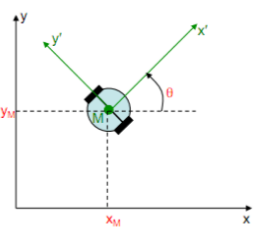
\includegraphics[width=0.39\textwidth]
		{Resources/PNG/transformationLocalGlobalBsp.png}
	\caption{}
\end{wrapfigure}

\paragraph{Kinematik} Die Kinematik ist die Lehre der Beschreibung von
Bewegungen von Punkten im Raum. Dabei werden die Größen Weg, Geschwindigkeit
und Beschleunigung betrachtet. Die Kinematik ist ein Teilgebiet der Mechanik.

\begin{description}
	\item[Kinematische Robotermodell] Zweiradbetriebener \\
		Kreisförmiger Roboter und Bewegung in der Ebene.
	\item[Lokales Koordinatensystem] An den Roboter verbunden mit Ursprung in der
		Mitte der Antriebsachse. Die x-Achse zeight in Richtung des Roboterfront.
	\item[Roboterposition im globalen Koordinatensystem] \hfill \\
		Globale Koordinaten $M(x_M, y_M)$ und der Drehung von $x'$ im Bezug zu $x$
		als Winkel $\theta$. \\
		$\Rightarrow$ Pose $p$ mit $p = \colvec{x_M\\y_M\\\theta}$

\end{description}

}

\subsection*{Transformation von lokalen in globale Koordinaten}
\vspace{-0.6cm}
{
\begin{wrapfigure}{r}{0.4\textwidth}
	\centering
	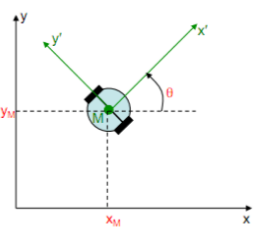
\includegraphics[width=0.25\textwidth]
		{Resources/PNG/transformationLocalGlobalBsp.png}
\end{wrapfigure}
\begin{align*}
	R_\alpha	&\mapsto\colvec{\sin\alpha&-\sin\alpha\\\sin\alpha & \cos\alpha} \\
	\vec{m} 	&= \colvec{x_M\\y_M} 																						 \\
	\vec{t}_g	&= R_\theta \cdot \colvec{x'\\y'} - \vec{m}
\end{align*}

}

\subsection*{Transformation von globalen in lokale Koordinaten}
\vspace{-0.6cm}
{
\begin{wrapfigure}{r}{0.4\textwidth}
	\centering
	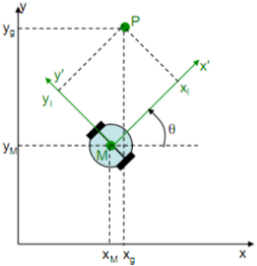
\includegraphics[width=0.25\textwidth]
		{Resources/PNG/transformationGlobalToLocal.png}
\end{wrapfigure}
\begin{align*}
	R_\alpha	&\mapsto\colvec{\sin\alpha&-\sin\alpha\\\sin\alpha & \cos\alpha} \\
	\vec{m} 	&= \colvec{x_M\\y_M} 																						 \\
	\vec{t}_l	&= R_{-\theta} \cdot \left(\colvec{x_g\\y_g} - \vec{m}\right)
\end{align*}

}

\section{Karten für statistische und dynamische Umgebungen}
Generell gilt: \textbf{Karten} sollen eine explizite Repräsentation des Raumes
sein.

Diese sind auf die Sensorik des Roboters zugeschnitten und nicht vorrangig für
den menschelichen Betrachter bestimmt.

\subsubsection*{Statische Umgebungen}
Basierend auf der Annahme, dass sich zwar der Zustand des Roboters innerhalb
der Umgebung, nicht jedoch die Umgebung selbst ändert.

$\Rightarrow$ Karte spiegelt die wirkliche Umgebung wieder.

\subsubsection*{Dynamische Umgebungen}
Objekte können ihre Lage oder ihren Zustand ändern. Dazu gehört das
verschwinden und auftauchen von bekannten oder unbekannten Objekten.

"Lernende" Karten sind ein fundamentales Problem in der mobilen Robotik

\subsection{Mapping Methoden}
Durch Koordinaten-Transformation kann zwischen den verschiedenen
Referenz-Frames beliebig ge\-wechselt werden.

\subsubsection{Weltzentriert}
Die Pose aller Objekte werden in der Umgebung in Bezug auf ein festes
Koordinatensystem repräsentiert.

Dies kann Indoor eine Zimmerecke sein und Outdoor ein globales
Koordinatensystem wie Längen- und Breitengrade, i.d.R. nutzen von
\textbf{WGRS}(World Geographic Reference System)

\subsubsection{Roboterzentriert}
Wird gebraucht um bspw. Kollisionen zu vermeiden. Diese nimmt als Bezugspunkt
den Roboter.

\subsection{Arten von Modellen}
Die wichtigste Form von Umgebungsmodellen für mobile Roboter sind
Umgebungskarten. Die folgende Ausführungen beziehen sich auf geeignet Karten
für \textbf{mobile, autonome Landfahrzeuge}

\begin{figure}[H]
	\begin{center}
		\includegraphics[scale=0.32]{Resources/PNG/MapTypes.PNG}
		\caption{Die verschiedenen Umgebungsmodelle}
		\label{fig:PNG/MapTypes.PNG}
	\end{center}
\end{figure}

\subsubsection{Arten von Umgebungsmodellen}
\begin{description}
	\item[Kontinuierliche metrische Karten] \hfill \\
	 	2D oder 3D bei denen jedes Objekt eine Koordinate erhält.
	\item[Diskrete  metrische Karten, Grid Maps] \hfill \\
		2D oder 3D bei der Raum in gleichmäßige oder ungleichmäßige Teile
		aufgeteilt wird. Ein Objekt wird mit einem dieser Teile assoziiert.
	\item[Hybrid Maps] \hfill \\
		z.B. Die Kontinuierliche metrische Anordnung von Grid Maps.
	\item[Topologische Modelle] \hfill \\
		Nur 2D bei der die Beziehung der Objekte zueinander im Vordergrund steht.
\end{description}

\subsection{Kontinuierliche Metrische Karten}
Metrische Lokalisierung beruht auf Ultraschall oder Laserscannern, bei der
eine exakte Beschreibung der Umgebung in 2D oder 3D möglich ist.

\textbf{Vorteil:} detailliertes Bild der Umgebung

\textbf{Nachteil:} große, unstrukturierte Datenmengen erschweren die
Pfadplanung

\subsection{Grid Maps - Rasterkarten}
{
\begin{wrapfigure}{r}{0.4\textwidth}
	\includegraphics[width=0.4\textwidth]{Resources/PNG/QuadTrees.png}
	\caption{oben: gleichmäßiges Gitter, unten: adaptives Gitter}
\end{wrapfigure}

Die Umwelt wird in gleichmäßiges Raster oder Grid zerlegt. Wobei für jede Zelle
mitgeführt wird ob sie belegt ist oder nicht. Dabei können je nach Modell
unterschiedliche Werte verwendet werden.
\begin{itemize}
	\item frei und belegt
	\item frei, belegt und Mischbelegung
	\item Belegungswahrscheinlichkeit
\end{itemize}
Notwendige Informationen sind z.B.:
\begin{itemize}
	\item x, y als Koordinaten (Zeile, Spalte) einer Zelle
	\item Sensordaten des Roboters
	\item Belegungswert
\end{itemize}
Dabei sind die Zellen unabhängig voneinander. Je höher die Messgenauigkeit der
Sensoren ist, desto kleiner können die Rasterelemente gewählt werden.

}

\subsubsection{Gleichmäßige Gitterstruktur vs. Adaptiver Gitterstruktur}
Für eine kompakte Notation können Grid Maps adaptive Unterteilt werden und im
2-dimensionalen Raum mit Quadtrees im 3-dimensionalen mit Octtrees gespeichert
werden.

\subsection{Adaptive Unterteilung}
\begin{enumerate}
	\item Ausgangszustand: Rechteck mit Hindernissen
	\item Fläche wird unterteilt in 4 Rechtecke gleicher Größe
	\item Jedes Rechteck wird rekursiv wieder in 4 Rechtecke unterteilt
		$\Rightarrow$ Quadtree
	\item Attributierung der Knoten:
		\begin{description}
			\item[Frei:] Rechteck enthält keinen Teil eines Hindernisses
			\item[Belegt:] Rechteck ist vollständig von Hindernis belegt
			\item[Gemischt:] Rechteck enhält nur Teile eines Hindernisses
		\end{description}
	\item Nur gemischte Knoten werden weiter unterteilt
\end{enumerate}
\subsubsection{Vorteile}
Schnell und leicht feststellbar, ob Punkt in einem Hindernis liegt

\subsubsection{Nachteile}
\begin{itemize}
	\item Konturen der Objekte und der Freiraum zwischen ihnen wird unpräzise repräsentiert
	\item Um die Datenfülle zu reduzieren, wird das Raster zu grob gewählt und dadurch ein möglicher Weg durch Mischpixel versperrt
\end{itemize}

{
\begin{wrapfigure}{r}{0.4\textwidth}
	\vspace{-1cm}
	\includegraphics[width=0.4\textwidth]{Resources/PNG/Trajektorie}
\end{wrapfigure}

\subsubsection{Weiterer Verwendungszweck}
Neben der reinen Lokalisierung können die Karten auch dazu verwendet werden
eine Fahrspur (Trakektorie) zu berechnen.

}

\subsubsection{Weitere Beispiele für Umgebungskarten}
\begin{itemize}
	\item Laserscan Karten
	\item Bildbasierte Karten
\end{itemize}

\subsection{Topologische Karten}
Bedingt geeignet zur Lokalisation, Haupteinsatzgebiet ist die Pfadplanung.
\begin{figure}[H]
	\begin{center}
		\includegraphics[width = \textwidth]{Resources/PNG/TopologischeKarte.PNG}
		\caption{}
		\label{fig:PNG/TopologischeKarte.PNG}
	\end{center}
\end{figure}
\begin{itemize}
	\item Modelle bilden einen \textbf{Graphen}
	\item \textbf{Knoten} entsprechen Orten oder Bereichen der Umgebung
	\item Beziehungen zwischen den Orten werden durch \textbf{Kanten} modelliert.
	\item Zwei Knoten sind durch eine Kante verbunden, wenn sie unmittelbar
		voneinander erreichbar sind.
	\item \textbf{Gewichte}: Maß für die Länge der Wege
	\item Ist die Länge der jeweiligen Wegstücke bekannt, lässt sich der
		kürzeste Weg finden.
\end{itemize}

\paragraph{Vorteile}
\begin{itemize}
	\item Kompaktheit
	\item Gute Skalierbarkeit für welträumige Umgebungen.
	\item Es gibt viele schnelle Algorithemn auf Graphen, die gut zur
		Pfadplanung eingesetzt werden können
\end{itemize}

\paragraph{Nachteil} Relevante Umgebungsmerkmale werden verdeckt. Landmarken
werden schwerer erkannt.

\subsection{Hybrid Maps}
\begin{itemize}
	\item Kombinieren metrische und topologische Ansätze
	\item Ermöglichen Lokalisation und Kantenerstellung mit hoher Präzision
	\item Erhalten die Kompaktheit der topologischen Ansätze
\end{itemize}

\paragraph{Abstraktions-basierter Ansatz}
\begin{itemize}
	\item Basis: konstruieren einer metrischen Karte der Umgebung
	\item $\Rightarrow$ aufbau einer kompakten topologischen Repräsentation
	\item \textbf{Vorteil} Effizient Planung eines Pfads zu einem gegebenen Ziel
		aufgrund der Abstraktion.
	\item Die zugrunde liegende metrische Karte wird für Relokalisation und
		Hindernisvermeidung benö\-tigt.
\end{itemize}

\section{Passive und Aktive Selbstlokalisierung}
\subsubsection*{Passive Verfahren}
\begin{itemize}
	\item bestimmen oder schätzen die Roboterposition mittels aktueller
		Sensorinformationen
	\item beeinflussen \textbf{nicht} die Bewegung und Orientierung des Roboters
	\item Lokalisierungsmodul beobachtet nur die Roboteroperationen
	\item Roboter bewegt sich zufällig hin und her bzw. führt die zu erledigende
		Aufgabe durch
\end{itemize}

\subsubsection*{Aktive Verfahren}
\begin{itemize}
	\item besitzen vollständige oder teilweise Kontrolle über die Bewegungen des
		Roboter und Ausrichtung der Sensoren
	\item fährt gezielt bestimmte Orte an um Mehrdeutigkeiten zwischen mehreren
		Orten aufzulösen
\end{itemize}

\section{Landmarken}
\subsubsection*{Definition}
Als Landmarken werden \textbf{eindeutig identifizierbare Charakteristiken der
Umwelt} bezeichnet, die von entsprechenden Sensoren erkannt werden können.

\paragraph{Landmarke}
\begin{itemize}
	\item ihre Position im Weltmodell ist bekannt
	\item sichtbar von unterschiedlichen Positionen aus
	\item erkennbar unter verschiedenen Belichtungen und Blickwinkeln
	\item relative Position bestimmbar
	\item stationär, oder dem Navigationsmechanismus musss die Bewegung bekannt
		sein
\end{itemize}

\paragraph{Vorteil} Navigation erfolgt mit der Umwelt selbst und nicht mittels
erechneter Daten

\subsubsection*{Natürliche Landmarken}
\begin{itemize}
	\item Werden nicht zum Zweck der Positionsbestimmung aufgestellt, können
		aber dafür verwendet werden
	\item Grundsätzlich Passiv
\end{itemize}

\subsubsection*{Künstliche Landmarken}
Markante Objekte, eigens zum Zwech der Positionsbestimmung in der Umgebung
installiert.

% !TEX root = ../Robotik.tex
\chapter{Fortbewegung, Lokalisierungsalgorithmen}
\section{Relative Lokalisierung}
\subsection{Dead Reckoning}
\begin{itemize}
	\item \textbf{Koppelnavigation oder Dead Reckoning} ursprünglich in der Nautik verwendet
	\item Mathematisches Verfahren - \textbf{Vorwärtskinematik} - zur Positionsbestimmung
	\item Ausgehend von einer Startposition ist es dem Navigator möglich, seine \textbf{aktuelle Position zu berechnen} aufgrund der \textbf{zurückliegenden bekannten Kurs- und Geschwindigkeitswerte}
\end{itemize}
\begin{figure}[H]
	\begin{center}
		\includegraphics[scale=0.7]{Resources/PDF/deadreckoning.pdf}
		\caption{}
		\label{fig:PDF/deadreckoning.pdf}
	\end{center}
\end{figure}
\begin{itemize}
	\item A sei ein gegebener Ausgangspunkt
	\item Radius wird angegeben der zur Abweichung proportional ist, bsp. hier 0,5m.
	\item Der Radius spiegelt die mit der Zeit kumulierte Ungenauigkeit wieder
	\item Eine mögliche Roboterposition ist dann innerhalb des Sektors gegeben der durch die Linien eingegrenzt wird
\end{itemize}
\paragraph{Vorteile}
\begin{itemize}
	\item einfache Implementierung
	\item leichte Interpretation der Daten
	\item unkomplizierte Bedienung
	\item passable Kurzstreckengenauigkeit
\end{itemize}
\paragraph{Nachteile}
\begin{itemize}
	\item Startposition muss bekannt sein
	\item Genauigkeit nimmt mit zunehmender Länge der befahrenen Strecke drastisch ab
\end{itemize}
\subsection{Odometrie}
Odometrie ist die Wissenschaft der Positionsbestimmung eines Fahrzeugs durch die Beobachtung seiner Räder.
\paragraph{Grundlegendes verfahren}
\begin{itemize}
	\item Sensoren an Rädern messen Drehbewegung
	\item \textbf{Relative Positionsbestimmung:} Die \textbf{Bestimmung der Position} erfolgt ausgehend von einer bekannten Position durch Berechnung des zurückgelegten Weges und anhand von Daten über den Roboter selbst.
	\item Es wird Inkrementalgebern die Anzahl $n$ der Radumdrehungen zwischen zwei Messpunkten gezählt. Aus dem bekannten Radumfang wird die wegdifferenz berechnet mit:
	\subitem $\Delta = \Pi \times d \times n $
	\item \textbf{Ausrichtung} kann durch differentiale Odometrie erfolgen: es werden z.B. die unterschiedlichen Entfernungen gemessen, die die linken und rechten Räder zurückgelegt haben.
\end{itemize}
\paragraph{Vorteile}
\begin{itemize}
	\item kostengünstig
	\item hohe Abtastraten
	\item passable Kurzzeitgenauigkeit
\end{itemize}
\paragraph{Fehlerquellen}
\begin{itemize}
	\item Fehlerhafte Messung des Raddurchmessers
	\item Raddurchmesser nicht gleich, Unrundheit des Radess
\end{itemize}
\paragraph{Fehlerberücksichtigung}
\begin{itemize}
	\item Die \textbf{Fehler} fließen in die Positionsdifferenz ein, werden zur letzten bekannten Position hinzuaddiert und \textbf{summieren sich mit jedem Messschritt}
	\item Fehlerellipse wächst mit zurückgelegtem Weg
	\item Odometrie als alleiniges verfahren nur für kurze Strecken geeignet
	\item Fehler lassen sich bei geringen Geschwindigkeiten und geringer Beschleunigung reduziern
\end{itemize}
\subsection{2D-Scanmatching}
\begin{itemize}
	\item Ausgangslage sind zwei Scans, ein Scan M (\textbf{Modell}) und ein zweiter Scan D (\textbf{Daten})
	\item Es wird eine Transformation des einen Scans berechnet und zwar so, dass beide optimal überlagert werden
	\item Die Transformationen bestehen nur aus einer Rotation und einer Translation
	\item Die Überlagerung ist optimal, wenn Punkte, die in der realen Szene nahe beieinander liegen, auch in den registrierten Messdaten nahe beieinander liegen.
	\item \textbf{Ziel}: Fehlerfunktion minimieren $\Rightarrow$ Abstände der Punkte des einen Scans zu ihren korrespondierenden Punkten des zweiten Scans
	\item Die Transformation des zweiten Scans entspricht dann der Bewegung des Roboters zwischen der Aufnahme der Daten; durch sukzessiven Vergleich kann damit die Bewegung des Roboters nachverfolgt werden
\end{itemize}
%TODO Rework this after understanding it
\paragraph{Iteratives Vorgehen}
\begin{figure}[]
	\begin{center}
		\includegraphics[scale=0.3]{Resources/PNG/2DScan.PNG}
		\caption{}
		\label{fig:PNG/2DScan.PNG}
	\end{center}
\end{figure}
\begin{itemize}
	\item \textbf{Annahme:} die korrespondierenden Punkte sind bekannt $\Rightarrow$ eine \textbf{Transformation} kann berechnet werden, die diese Mengen aufeinander abbildet
	\item \textbf{Beispiel} zwei Scans mit einer Poseänderung des zweiten um $(4cm, 1cm, 10 \deg)^T$ beide Scans sehen dieselben Raumpunkte p1 und p2
	\item Obige Annahme i.d.r. nicht erfüllt $\Rightarrow$ \textbf{nicht eindeutig zu bestimmen, welche Punkte zwischen den beiden Scans korresponideren}
	\item \textbf{Lösung}: \textbf{iteratives Vorgehen}, bei dem zunächst eine \textbf{Schätzung} der Punktepaarung stattfinden und die Pose des zweiten Scans unter dieser Paarung optimiert wird.
	\item Iterativ werden mit dem transformierten Scan neue Punktepaare berechnet, bis ein Abbruchkriterium erfüllt ist, d.h. bis sich die Transformation zwischen zwei Schritten nich mehr signifikant ändert
\end{itemize}
\paragraph{Transformationsberechnung}
\begin{itemize}
	\item \textbf{Gesucht}: Mögliche Menge von Translationen und Rotationen, unter denen ein korrektes Matching möglich ist.
	\item $(t_x, t_z, \theta)^T$, die eine Translation um $t_x$ in x-Richtung und $t_z$ entlang der Z-Achse durchführt, sowie eine Rotation um den Winkel $\theta$
	\item Der Scan M besteht aus einer Menge von Punkten ($m_i$)i=1,2...N
	\item Der Scan D besteht aus einer Menge von Punkten ($D_i$)i=1,2...N
\end{itemize}
\paragraph{Minimum der Funktion}
$E(\theta, t)=\sum_{i=1}^{N}\left\|p_{i}-\left(\boldsymbol{R}_{\theta} \boldsymbol{p}_{i}^{\prime}+\boldsymbol{t}\right)\right\|^{2}$
\paragraph{Transformation zur mimierung der Fehlerfunktion E}
Folgende Transformation mit ggb. Parametern minimiert die Fehlerfunktion:\\
$\theta=\arctan \left(\frac{S_{z x^{\prime}}-S_{x z^{\prime}}}{S_{x x^{\prime}}+S_{z z^{\prime}}}\right)$
\\
Hierbei ist \\
$t_{x}=c_{x}-\left(c_{x}^{\prime} \cos \theta-c_{z}^{\prime} \sin \theta\right)$ und \\
$t_{z}=c_{z}-\left(c_{x}^{\prime} \sin \theta+c_{z}^{\prime} \cos \theta\right)$
%TODO Look at BSP 26 / 28

% !TEX root = ../Robotik.tex
\chapter{Navigation}
\section{Bekanntes vs. unbekanntes Terrain}
Man unterscheidet zwischen Algorithmen für:
\begin{itemize}
	\item \textbf{bekannte Umgebung:} auch während der Fahrt ändert sich die
		Umgebung nicht
	\item \textbf{unbekannte Umgebung:} entweder vollständig oder Teilweise
		unbekannte Umgebung
\end{itemize}

Ist das Gebiet \textbf{vollständig bekannt}, lässt sich die Suche mittels eines
Graphen lösen. Ansonsten erfolgen die Berechnungen auf lokalen
Teilinformationen von Sensoren mit denen \textbf{inkrementelle Anpassungen}
vorgenommen werden.

\section{Navigation in unbekanntem Terrain}
\subsection{Konturverfolgung}
Eine \textbf{Freiraumfahrt} d.h. eine Fahrt durch ein Gelände, dessen
Raum möglichst weit und frei von Hindernissen ist, ist nicht immer Zielführend.

Lösung: \textbf{Konturverfolgung}
\begin{itemize}
	\item Roboter wird nah an einem Objekt (Wand, Hinderniss) entlang bewegt
	\item Es sollte möglichst ein gegebener Abstand $d$ eingehalten werden
\end{itemize}

\begin{lstlisting}[language=bash, caption={Regelung des Abstands $d$}]
if (Distance to Wall > d) then
	turn to wall
fi

if (Distance to Wall < d) then
	turn away from wall
fi

if (Distance to Wall == d) then
	Drive straight ahead
fi
\end{lstlisting}

\pagebreak
\subsection{Bug1 Algorithmus}
{
\begin{wrapfigure}{r}{0.4\textwidth}
	\vspace{-1cm}
	\includegraphics[width=0.4\textwidth]{Resources/PNG/Bug1.PNG}
	\caption{Bug1 Algorithmus Route}
	\label{fig:PNG/Bug1.png}
\end{wrapfigure}
\paragraph{Vorraussetzungen}
\begin{itemize}
	\item Bewegung auf einer geraden Linie
	\item Konturverfolgung
	\item Roboter benötigt einen Sensor zur Erkennung eines "Kontakts" mit einem
		Hindernis
	\item Roboter kann die Distanz zwischen zwei Punkten x und y messen
	\item der Arbeitsraum ist begrenzt
\end{itemize}

}

\paragraph{Algorithmus}
\begin{lstlisting}[language=c++, caption={}]
while ( noch nicht am Ziel ) {
	try {
		Folge gerader Linie zum Ziel
	} catch ( HindernisKontakt kontaktpunkt ) {
		Umfahre das Hindernis bis wieder bei $kontaktpunkt
		leavepoint = Punkt mit Lot vom Hindernis zum Ziel
		Fahre zu $leavepoint
	}
}
\end{lstlisting}

\paragraph{Exception}
Schneidet die Linie von $q1^L$ zum Ziel das \textbf{aktuelle Hindernis} gibt
es keine Lösung
\begin{figure}[H]
	\begin{center}
		\includegraphics[scale=0.4]{Resources/PNG/Exception1.PNG}
		\caption{}
		\label{fig:PNG/Exception1.PNG}
	\end{center}
\end{figure}

\subsection{Bug2-Algorithmus}
Schnellere Variante zu Bug1, da Hindernis nicht komplett umrundet wird.
Eventuell keine mögliche Lösung wie bei Bug1. \textbf{Backtracking} und
damit Veränderung der Umfahrichtung eines Hindernisses können helfen.

\pagebreak

\begin{lstlisting}[language=c++, caption={Algorthmus ohne Backtracking}]
/**
 * Start S
 * Ziel T
 * Derzeitige Position P = S
 * Umfahrrichtung = rechts
 */
Konstruiere Strecke ST
while (nicht bei T) {
	try {
		Fahre auf ST
	} catch (HindernisKontaktPunkt H) {
		while (P == Schnittpunkt mit ST && len(PT) < len(HT)) {
			Umfahre das Objekt rechtsherum
		}
	}
}
\end{lstlisting}

\subsection{Bug3-Algorithmus}
Unterschied zu Bug2 ist, dass er nicht der Strecke ST strikt folgt sondern
jede Möglichkeit nutzt näher ans Ziel T zu kommen. Auch hier Problematik keine
Lösung zu finden und Verbesserung durch Backtracking möglich.

\begin{lstlisting}[language=c++, caption={Algorthmus ohne Backtracking}]
/**
 * Start S
 * Ziel T
 * Derzeitige Position P = S
 * Umfahrrichtung = rechts
 */
while (nicht bei T) {
	try {
		Fahre zu T
	} catch (HindernisKontakt) {
		while (PT nicht frei) {
			Umfahre das Objekt rechtsherum
		}
	}
}
\end{lstlisting}

\subsection{Labyrinthe}
\subsubsection{Grundprobleme}
\begin{itemize}
	\item Es wird davon ausgeangen, dass der Roboter berühren oder "sehen" kann
	\item Zwei grundlegend Hauptprobleme:
		\begin{itemize}
			\item Einen \textbf{Weg in ein Labyrinth} finden, um einen bestimmten
				Gegenstand oder \textbf{Schatz zu erreichen} sowie den \textbf{Rückweg
				zum Eingang}
			\item \textbf{Flucht aus einem Labyrinth} von einer unbekannten Stelle
				aus.
		\end{itemize}
	\item Enger Zusammenhang zwischen Labyrinth und Graphen $\Rightarrow$ Jeder
		Korridor:= Kante und jede Kreuzung:= Knoten
	\subitem Bei bekanntem Labyrinthe $\Rightarrow$ Suchproblem in Bäumen
\end{itemize}

\subsubsection{Verlassen eines Labyrinths mit Pledge Algorithmus}
\textbf{Grundidee} Vorsichtig geradeaus bis man auf ein Hindernis trifft und
dann mit der "linken" Hand immer an der Wand entlang bis zum Ausgang.

\textbf{Problem} Enthält das Labyrinth eine Säule, läuft man für immer im
Kreis

\textbf{Lösung} Man folgt der Wand nur solange, bis man wieder in die alte
Richtung schaut.

\textbf{Allgemeingültige Lösung} Drehungen beim Abbiegen an den Ecken
mitzählen. Bei jeder Linksdrehung wird der Umdrehungszähler inkrementiert, bei
jeder Rechtsdrehung dekrementiert.
\begin{itemize}
	\item Bewege den Roboter geradeaus bis eine Wand erreicht ist
	\item Folge der Wand bis Umdrehungszähler 0 ist
\end{itemize}

\subsubsection{Verlassen eines Labyrinths mit Ariadenfaden}
\textbf{Ziel}: einen Weg zu einem versteckten Ziel im Labyrinth sowie wieder
zurück zum Eingang finden ohne dass eine Karte des Labyrinths bekannt ist

\textbf{Idee}: Wenn man ein Labyrinth betritt Faden ausrollen $\Rightarrow$
zurückverfolgen bringt einen zurück zum Eingang.

\textbf{Vorraussetzungen und grundsätzliches Vorgehen}
\begin{itemize}
	\item einer Wand folgen
	\item Umdrehen
	\item Kreuzungen erkennen
	\item Ziel erkennen
	\item Faden auslegen und wieder einsammeln
	\item Faden am Boden erkennen
	\item Faden zur nächsten Kreuzung folgen
\end{itemize}

\subsubsection{Tarry und Tremaux Algorthmus}
\begin{itemize}
	\item Beispiel für klassische Tiefensuche
	\item Richtung, in der sich das zu suchende Objekt befindet ist unbekannt.
	\item Graph kann zyklen enthalten
	\item Es wird ein zyklisch gerichteter Graph durch jede Kante konstruiert,
		wobei jede Kante nur einmal pro Richtung besucht wird
\end{itemize}

\textbf{Algorithmus:}
\begin{itemize}
	\item Starte willkürlich an einem Knoten
	\item Folge einem möglichen Pfad, markiere die Kante, in welcher Richtung
		sie betreten worden ist
	\item Sind alle Kanten schon betreten, eine auswählen, die bis jetzt nur in
		die Gegenrichtung betreten wurde.
	\item Trifft man auf eine Sackgasse oder einen schon besuchten Gang, zurück
		zur letzten Kreuzung
	\item Es darf kein Pfad betreten werden, der schon in beide Richtungen
		besucht wurde.
	\item Algorithmus ist beendet, wenn der Startpunkt erreicht wird.
\end{itemize}

\section{Pfadplanung für mobile Roboter in bekanntem Terrain}
Ziel der Navigation ist es, ein Fahrzeug in der Umwelt zu bewegen.
Dies beinhaltet drei Unteraufgaben:
\begin{description}
	\item[Global Pfadplanung]
	\begin{itemize}
		\item \textbf{Vorraussetzung}: es gibt eine Karte
		\item suche eines Pfades von einem Start- zu einem Zielpunkt in vorhandenem Umgebungsmodell
		\item evtl. auch Suche nach Pfad mit geringsten Kosten
		\item Kompletter Pfad beschrieben durch Menge von Punkten
	\end{itemize}
	\item[Lokale Pfadplanung] berücksichtigt Fahrzeug-Dimension und kinematische
		Einschränkungen
	\item[Path Control] generiert geeignet Steuerbefehle, um den vorberechneten
		Pfad zu folgen
\end{description}

\subsection{Konfigurationsraum}
Summe aller Konfigurations-Hindernisse bildet den \textbf{Konfigurationsraum}.
Dieser ist eine Datenstruktur, die es dem Roboter ermöglicht, die \textbf{
Position und Orientierung von Hindernissen} in der Umgebung zu definieren. Der
Konfiguration dient somit als \textbf{Basis der Webplanung}.

\paragraph{Herleitung}
\begin{itemize}
	\item Abmesungen, Form, Bewegungsmöglichkeiten des Roboters werden für die
		Erstellung des Konfigurationsraums benötigt
	\item Konfiguration $q$ eines Roboters beschreibt Lage und Ausrichtung im
		Bezugssystem des Umgebungsmodells
	\item Im zweidimensionalen Raum kann Position in $x,y$-Ebene und Orientierung
		ausgedrückt werden
	\item Konstruktionsbedingt sind einige Konfigurationen für den Roboter in
		seiner Umgebung nicht zulässig
	\item Problem; einfachere Darstellung:
	\subitem Roboter als Punkt angenommen
	\subitem Abmessungen des Roboters + Objektabmessungen $\Rightarrow$
		Konfigurations-Hindernisse
\end{itemize}
\begin{figure}[H]
	\begin{center}
		\includegraphics[scale=0.5]{Resources/PNG/KonfigurationsHindernisse.PNG}
		\caption{}
		\label{fig:PNG/KonfigurationsHindernisse.PNG}
	\end{center}
\end{figure}

\paragraph{Repräsentationen}
\begin{itemize}
	\item Graphen mit Knoten
	\item Reguläre Gitter
	\item Quad-Bäume oder Octal-Bäume
	\item Voronoidiagramme
\end{itemize}

\section{Algorithmen und Methoden}
Für die folgenden Algorithmen und Methoden wird ausgeganen, dass Hindernisse
bekannt sind und weder Position noch Form ändern.

\paragraph{Zellzerlegungen} Das Umgebungsmodell wird in sich nicht überlappende
Zellen unterteilt, die als besetzt oder frei markiert sind

\paragraph{Straßenkartenmethoden oder Roadmaps}
Eine Roadmap ist ein Graph mit Knoten und Kanten, bei dem alle befahrbaren
Wege hinterlegt sind. Daraus kann ein kollisionsfreier Pfad vom Start- zum
Zielpunkt erstellt werden.

Auf dieses Netzwerk können Standardmethoden der Graphentheorie, wie sie auch in
der Autonavigation Verwendung finden, andwendet werden:
\begin{itemize}
	\item kürzeste Wegsuche mit A*, Dijkstra
	\item Wegsuche mit Umgehung von Hindernissen mit dem
		\textbf{Sichtbarkeitsgraph}
	\item Wegsuche mittels eines \textbf{Voronoigraphen},
		\textbf{Voronoidiagramms}
\end{itemize}

\paragraph{Potentialfeldmethoden} beinhalten die physikalische Simulation des
Roboters als Partikel in einem Feld.

\subsection{Dijkstra}
\begin{lstlisting}[language=c++]
/**
 * PriorityQueue Open
 */
struct Knoten {
	int cost
	Knoten* predecessor
}
Knoten start = {0, null};
push start on Open

while (Open is not empty) {
	Knoten n = pop lowest cost from Open
	if (ist n Ziel?) {
		konstruiere weg
		return sucess
	}
	for (Knoten nx : nachfolger von n) {
		newcost = n.cost + wegkosten von n nach nx
		if (n ist in Open && nx.cost <= newcost) {
			continue;
		}
		nx.predecessor = n
		nx.cost = newcost
		if (nx is not in Open) {
			push nx in Open
		}
	}
}
return failure
\end{lstlisting}

\subsection{A*}
\begin{lstlisting}[language=c++]
/**
 * PriorityQueue Open
 * List Closed
 */
struct Knoten {
	int total 					// total cost
	int est							// estimated cost
	int known 					// known cost
	Knoten* predecessor
}
Knoten start;
start.total = 0;
start.est = GoalDistEstimate(start);
start.known = start.total + start.est;
start.predecessor = null;

push start on Open

while (Open is not empty) {
	Knoten n = pop lowest total cost from Open
	if (ist n Ziel?) {
		konstruiere weg
		return sucess
	}
	for (Knoten nx : nachfolger von n) {
		newcost = n.known + wegkosten von n nach nx
		if ((n ist in Open || n ist in Closed) && nx.known <= newcost) {
			continue;
		}
		nx.predecessor = n
		nx.known = newcost
		nx.est = GoalDistEstimate(nx)
		nx.total = nx.known + nx.est
		if (nx is in Closed) {
			remove nx from Closed
		}
		if (nx is not in Open) {
			push nx in Open
		}
	}
	push n onto Closed
}
return failure
\end{lstlisting}

\subsection{Wegsuche mit dem Sichtgraph-Algorithmus}
\paragraph{Visibility Map}
\begin{itemize}
	\item enthält Eckpunkte von Polygonen, den Ecken der Hindernisse
	\item zwei Knoten der Visibility Map teilen eine Kante, wenn die beiden Eckpunkte voneinander in Sichtweite sind
\end{itemize}
\paragraph{Visibility Graph}
\begin{itemize}
	\item ist die einfachste Visibility Map
	\item Knoten umfassen: \textbf{Startknoten}, \textbf{Zielknoten} und alle Eckpunkte der Hindernisse
	\item die Kanten sind Liniensegmente, die zwei Knoten in Sichtweite verbinden
	\item Hinderniskanten sind Teil des Sichtgraphen
\end{itemize}
\paragraph{Sichtgraphenalgorithmus}
\begin{itemize}
	\item verbinde \textbf{Start-}, \textbf{Zielpunkte} und die \textbf{Ecken} der Hindernisse durch Geraden, die nicht durch Hindernisse laufen dürfen
	\item Ergebnis ist ein Graph, dessen Knoten Orte sind und dessen Kanten mögliche Wegstücke zwischen diesen Knoten darstellen
	\item Kanten sind gewichtet mit der Entfernung zwischen den Knoten
	\item gesucht: Menge der möglichen Geraden, die den Startpunkt auf dem kürzesten Weg mit dem Zielpunkt verbindet
	\item \textbf{Nachteil}: führt unmittelbar an Hindernissen entlang, enthält noch viele nutzlose Kanten
\end{itemize}
\begin{figure}[H]
	\begin{center}
		\includegraphics[scale=0.5]{Resources/PNG/SichtGraphAlgorithmus.PNG}
		\caption{}
		\label{fig:PNG/SichtGraphAlgorithmus.PNG}
	\end{center}
\end{figure}
\paragraph{Reduzierter Visibility Graph}
Definition von \textbf{unterstützenden} und \textbf{trennenden} Kanten:
\begin{itemize}
	\item \textbf{unterstützende Kante:} Tangente zu zwei Hindernissen, so dass die Hindernisse auf derselben Seite der Linie liegen
	\item \textbf{trennende Kante:} Tangente zu zwei Hindernissen, so dass die Hindernisse auf gegenüberliegenden Seiten der Tangente liegen
\end{itemize}
Der reduzierte Sichtgraph besteht nur aus unterstützenden und trennenden Kanten.
\begin{figure}[H]
	\begin{center}
		\includegraphics[scale=0.4]{Resources/PNG/SichtGraphReduziert}
		\caption{}
		\label{fig:PNG/SichtGraphReduziert.PNG}
	\end{center}
\end{figure}
\paragraph{Konstruktion des Graphen}
\begin{itemize}
	\item Alle Liniensegmente $vv_i$ mit $v != v_i$ müssen getestet werden, ob sie keinen Schnittpunkt mit einer Kante eines Hindernisses haben
	\item \textbf{Nachteil}: Komplexität O($n^3$)
	\item \textbf{Effizienter}: Plane Sweep Algorithmus mit Komplexität O($n^2 log n$)
\end{itemize}
\paragraph{Algorithmus}
\begin{itemize}
	\item \textbf{Input}: A  set of vertices ${v_i}$ (whose edges do not intersect) and a vertex $v$
	\item \textbf{Output}: A subset of vertices from ${v_i}$ that are within line of sight of $v$
\end{itemize}
\begin{itemize}
	\item For each vertex $v_i$, calculate $\alpha$, the angle from the horizontal axis to the line segment $\overline{vv_i}$
	\item Create the vertex list $\epsilon$, containing the $\alpha_i$'s sorted in increasing order.
	\item Create the active list $\mathcal{S}$, containing the sorted list of edges that intersect the horizontal half-line emanating from v.
	\item \textbf{For all} $\alpha_i$ \textbf{do}
	\subitem if $v_i$ is visible to $v$ \textbf{then}
	\subsubitem Add the edge ($v, v_i$) to the visibility graph.
	\subitem \textbf{end if}
	\subitem \textbf{if} $v_i$ is the beginning of an edge, E, not in $\mathcal{S}$ \textbf{then}
	\subsubitem Insert the \textit{E} into $\mathcal{S}$
	\subitem \textbf{end if}
	\subitem \textbf{if} $v_i$ is the end of an edge in $\mathcal{S}$ \textbf{then}
	\subsubitem Delete the edge from $\mathcal{S}$
	\subitem \textbf{end if}
	\item \textbf{end for}
\end{itemize}
\subsection{Voronoi-Diagramme}
\paragraph{Allgemeines Voroni-Diagramm}
\begin{itemize}
	\item Eine Fläche wird willkürlich mit Punkten besetzt $\Rightarrow$ erzeugt Polygonflächen
	\item Alle punkte einer Polygonfläche liegen am nähesten zu dem Punkt der im Zentrum dieses Polygons liegt
	\item Jede Zelle hat genau ein Zentrum
	\item Die Punkte des Gebiets, die zu mehereren Zentren den gleichen Abstand haben, bilden die Grenze zwischen den einzelnen Zellen
	\item Als abstandsfunktion wird der Euklidische Abstand verwendet:
	\subitem $dist(p,q) ) = \sqrt{(p_x-q_x)^2 + (p_y-q_y)^2}$
	\item Das Voronoi-Diagramm ist die Menge solcher Grenzlinien
\end{itemize}
\begin{figure}[H]
	\begin{center}
		\includegraphics[scale=0.4]{Resources/PNG/Polygon.PNG}
		\caption{}
		\label{fig:PNG/Polygon.PNG}
	\end{center}
\end{figure}
Immer dann gut einsetzbar, wenn ungenaue Sensoren zur Verfügung stehen oder die Umwelt ungenau geometrisch modelliert wurde oder sich dynamisch ändert.
\paragraph{Generalisierte Voronoi-Diagramme}
\begin{itemize}
	\item Bei der Navigation von Robotern wird eine verallgemeinerte Version des Voronoi Diagramms verwendet, das sogenannte \textbf{generalisierte Voronoi Diagramm}(GVD)
	\item \textbf{Generalisierung} betrifft die \textbf{Form der Zentren} und die Art der \textbf{Abstandsfunktion}
	\item \textbf{Zentren} können aus \textbf{komplexeren Formen} wie Linien, Kurven oder Polygonen \textbf{statt Punkten} bestehen
	\item Objekten der Umgebung werden als \textbf{Voronoi-Zentren} behandelt
	\item Die Menge aller \textbf{Voronoi-Kanten}, das GVD, stellt mögliche \textbf{kollisionsfreie Wegstücke} dar
	\item Falls sich der Roboter entlang einer \textbf{Voronoi-Kante} bewegt, kann er nicht mit Hindernissen kollidieren
	\item Beliebtes Verfahren zur Repräsentation des Konfigurationsraumes und Erzeugung eines Graphen.
	\item Punkte an denen sich \textbf{Voronoi-Kanten} schneiden, werden zu \textbf{Voronoi-Knoten}
\end{itemize}
\begin{figure}[H]
	\begin{center}
		\includegraphics[scale=0.6]{Resources/PNG/Voronoi.PNG}
		\caption{}
		\label{fig:PNG/Voronoi.PNG}
	\end{center}
\end{figure}
Start- und Zielpunkt des gesuchten Weges liegen normalerweise nicht auf dem Diagramm.
Diese beiden Punkte werden mit der nächstliegenden Kante verbunden.
Die Berechnung des optimalen Weges auf dem Voronoi-Diagram kann mit üblichen Graphenalgorithmen vorgenommen werden.
\subsection{Navigation in einer Rasterkarte}
\begin{itemize}
	\item Die Karte ist durch ein binäres Raster mit freiem Platz und Hindernissen gegeben.
	\item Das Raster wird ausgehend vom Startpunkt: \textbf{geflutet} $\Rightarrow$ Füllt den gesamten Hindernisfreien Raum
	\item In jeder Iteration haben alle Pixel auf einer Wellenfront dieselbe Pfadlänge im Raster bezogen auf den Zielpunkt
	\item Backtracking vom Zielpunkt zurück zum Startpunkt und erstellt dabei eine Liste der passierten Rasterpunkte
	\item Gewählt kann jeder Punkt im Raster werden, dessen Wert eins geringer ist, als der aktuell betrachtete
	\item Trifft dies auf mehrere Punkte zu, wird willkürlich einer gewählt
\end{itemize}
\begin{figure}[H]
	\begin{center}
		\includegraphics[scale=0.6]{Resources/PNG/RasterKarte.png}
		\caption{}
		\label{fig:PNG/RasterKarte.png}
	\end{center}
\end{figure}
\paragraph{Fluten der Karte}
\begin{itemize}
	\item Ein \textbf{Rasterpunkt} besitzt vier Nachbarpunkte: \enquote{N}, \enquote{O}, \enquote{S} , \enquote{W}
	\item Ein Rasterpunkt z ist mit 0 für freien Raum belegt und -1 für ein Hindernis
	\item Wenn ein Rasterpunkt eine Nummer erhalten hat, behält er diese Nummer
	\item Der Algorithmus benutzt aus Performancegründen zwei Stacks $S_0$ und $S_1$, die abwechselnd gefüllt und geleert werden. Die Stacks sind anfangs leer
\end{itemize}
\begin{figure}[H]
	\begin{center}
		\includegraphics[]{Resources/PNG/Flooding.PNG}
		\caption{}
		\label{fig:PNG/Flooding.PNG}
	\end{center}
\end{figure}
\paragraph{Alternativer Wave Front Planer}
Siehe Ursprungsfolie Kapitel 5, Seite 29/30
\subsection{Potentialfeld methode}
\paragraph{Grundidee}
\begin{itemize}
	\item Vorbild: \textbf{Elektrisches Feld}
	\item Start- und Zielpositionen, die Positionen aller Hindernisse müssen bekannt sein.
	\item Der \textbf{Zielpunkt und Freiräume} erhalten ein \textbf{anziehendes Potential}
	\item Der \textbf{Startpunkt, die Hindernisse} und Wände erhalten ein \textbf{abstoßendes Potential}
	\item Es wird eine Karte generiert mit virtuell anziehenden und abstoßenden Kräften
	\item Kräfte nehmen linear mit dem Abstand zu den Objekten ab.
	\item \textbf{Ein Objekt bewegt sich nach der Methode des steilsten Abstiegs im Potentialfeld auf das Ziel zu.}
\end{itemize}
\begin{figure}[H]
	\begin{center}
		\includegraphics[scale=0.5]{Resources/PNG/PotentialFeld.PNG}
		\caption{}
		\label{fig:PNG/PotentialFeld.PNG}
	\end{center}
\end{figure}

% !TEX root = ../Robotik.tex
\chapter{Probabilistische Methoden und Kartierungen}
\section{Problemstellung}

\begin{description}
	\item[Sensordaten] Roboter empfängt regelmäßig Sensordaten, jedoch mit
		Unsicherheit behaftet.
	\item[Steuerdaten] Roboter führt regelmäßig Bewegungen mit Steuerdaten $u_k$
		durch, aber diese entsprechen nicht exakt den vorgegebenen Steuerdaten.
	\item[Position und Umgebungsmodell] Position schätzt seine globale Position
		aufgrund der Sensor- und Steuerdaten in seiner Umgebungskarte, jedoch auch
		mit Unsicherheit behaftet
\end{description}

\section{Modellierung von Unsicherheit}
Die Unsicherheiten werden mit Wahrscheinlichkeiten modelliert. So kann der
Zustand von dynamsichen Systemen probabilistisch geschätzt werden.

\paragraph{Beispiel: Localization beim Roboter}
Dabei wird die Position ermittelt an der sich der Roboter am
wahrscheinlichsten befindet. Die Lokalisierung wird somit zu einem
Wahrscheinlichkeitsdichte Problem bei dem alle vorangegangenen Sensorwerte
berücksichtigt werden.

\section{Umgebungsmodellierung mit Occupancy Grids}
\subsection{Satz von Bayes}
\begin{align*}
	p(A) &= \text{Wahrscheinlichkeit das die Aussage } A \text{ zutrifft} \\
	P(A|B) &= \text{Wahrscheinlichkeit, dass } p(A) \text{ unter der
									Voraussetzung das }B\text{ gilt} \\
  P(A|B) &= p(B|A) * \frac{p(A)}{p(B)}
\end{align*}

\subsection{Evidence Grids (Beweisraster)}
\textbf{Problem}: reale Sensordaten erhalten häufig Rauschen.
Rauschen bei  Sensordaten führt zu Abweichungen des Idealwerts $\Rightarrow$
schwerwiegende Fehler.

Im Gegensatz zu Occupancy Grids nutzen Evidence Grids keine Binärwerte um die
Belegung darzustellen. Sie sammeln Beweismittel und geben die
Wahrscheinlichkeit für die Belegung jeder Zelle an:
$$
	Z(x,y) = p(Z_{x,y,belegt} | Sensorwert) / p(Z_{x,y,frei} | Sensorwert)
$$
Da die Wahrscheinlichkeit für die Belegung unter einem bestimmten Sensorwert
schwer zu berechnen ist wird der Satz von Bayes benutzt:
$$
	Z(x,y) = \frac{p(Sensorwert | Z_{x,y,belegt}) * p(Z_{x,y,belegt})}
								{p(Sensorwert | Z_{x,y,frei}) * P(Z_{x,y,frei})}
$$
Beim Start der Erstellung wird angenommen, dass die Wahrscheinlichkeit für die
Belegung einer Zelle bei 50\% liegt. Dannach wird die Wahrscheinlichkeit
fortlaufend mit den aktuellen Sensorwerten aktualisiert.

Die direkte Anwendung des Bayessischen Filters auf das
Selbstlokalisierungsproblem ergibt sich die sogenannte \textbf{Markov-
Lokalisierung}

\section{Bayes-Filter Algorithmus}
Der Vertrauenszustand (\textbf{belief}) spiegelt internes Wissen des Roboters
über den Zustand seiner Umgebung wieder.

\subsection{Algorithmus}
Ein Rekursiver Algorithmus der aus dem vorangegangenen Status den neuen
berechnet:
\begin{align*}
	z_t &= \text{Observationsmesswert, aktuelle Sensorwerte der Umgebung} \\
	u_t &= \text{Aktionsmesswert, aktuelle Zustandsänderungen im Interval }
		]t-1, t] \\
	x_t &= \text{Zustand zum Zeintpunkt }t \\
	bel(x_t) &= p(x_t | Z_{1:t}, u_{1:t}) \\
\end{align*}

Eine Vorhersage liefert, da dort die aktuellen Sensordaten noch nicht
berücksichtigt werden:
$$
	\overline{bel}(x_t) = p(x_t | z_{1:t-1}, u_{1:t})
$$
\begin{center}
	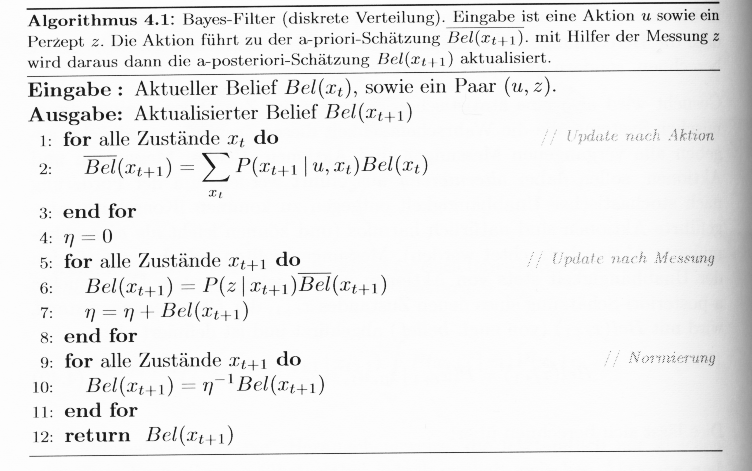
\includegraphics[scale=0.4]{Resources/PNG/hertzberg-132-bayes-algorithmus.png}
\end{center}

\subsection{Beispiel Aufgabenstellung}
Roboter schätzt den Zustand einer Tür mittels einer Kamera, er macht eien
Beobachtung z.

Annahmen:
\begin{itemize}
	\item Türe kann nur offen oder geschlossen sein
	\item Nur der Roboter kann den Zustand der Tür ändern
\end{itemize}

Der Roboter kennt den Zustand der Tür nicht $\Rightarrow$ Gleichverteilung
\begin{align*}
	&bel(X_0 = open) &= 0.5 \\
	&bel(x_0 = closed) &= 0.5
\end{align*}

Verrauschen der Sensoren $\Rightarrow$ bedingt Wahrscheinlichkeit
\begin{align*}
	&p(Z_t = sense\_open | X_t\, is\_open) = 0.6 \\
	&p(Z_t = sense\_closed | X_t\, is\_open) = 0.4 \\
	&p(Z_t = sense\_open | X_t\, is\_closed) = 0.2 \\
	&p(Z_t = sense\_closed | X_t\, is\_closed) = 0.8
\end{align*}

Der Roboter kann die Tür öffnen
\begin{align*}
	&p(X_t = is\_open | U_t = push, X_{t-1} = is\_open) = 1 \\
	&p(X_t = is\_closed | U_t = push, X_{t-1} = is\_open) = 0 \\
	&p(X_t = is\_open | U_t = push, X_{t-1} = is\_closed) = 0.8 \\
	&p(X_t = is\_closed | U_t = push, X_{t-1} = is\_closed) = 0.2
\end{align*}

Der Roboter tut nichts
\begin{align*}
	&p(X_t = is\_open | U_t = nothing, X_{t-1} = is\_open) = 1 \\
	&p(X_t = is\_closed | U_t = nothing, X_{t-1} = is\_open) = 0 \\
	&p(X_t = is\_open | U_t = nothing, X_{t-1} = is\_closed) = 0 \\
	&p(X_t = is\_closed | U_t = nothing, X_{t-1} = is\_closed) = 1
\end{align*}

\subsection{Beispiel Rechnung}
Für $t=1$ mit $u_1$ = nothing und $z_1$ = sense_open:
\begin{align*}
	\overline{bel}&(x_1 = open) = \\
		&p(x_1 = open | u = nothing, x_0 = open)bel(x_0 = open) + \\
		&p(x_1 = open | u = nothing, x_0 = closed)bel(x_0 = closed) \\
		&= 1 * 0.5 + 0 * 0.5 = 0.5 \\
	\overline{bel}&(x_1 = closed) = \\
		&p(x_1 = closed | u = nothing, x_0 = open)bel(x_0 = open) + \\
		&p(x_1 = closed | u = nothing, x_0 = closed)bel(x_0 = closed) \\
		&= 0 * 0.5 + 1 * 0.5 = 0.5 \\
	\eta = 0: bel&(x_1 = open) =  \\
		&p(z = sense_open | x_1 = open)\overline{bel}(x_1 = open) \\
		&= 0.6 * 0.5 = 0.3 \\
	\eta = 0.3: bel&(x_1 = closed) = \\
		&p(z = sense_open | x_1 = closed)\overline{bel}(x_1 = closed)\\
		&= 0.2 * 0.5 = 0.1 \\
	\eta = 0.4: bel&(x_1 = open) = bel(x_1 = open) * \eta^-1
		= 0.3 * 0.4^-1 = 0.75 \\
	bel&(x_1 = closed) = bel(x_1 = closed) * \eta^-1
		= 0.1 * 0.4^-1 = 0.25
\end{align*}

{
\begin{wrapfigure}{r}{0.4\textwidth}
	\includegraphics[width=0.4\textwidth]{Resources/PNG/MarkovAlgorithmus.PNG}
\end{wrapfigure}
\section{Markov Lokalisierung}
Bei der Markov Lokalisierung geht von der Annahme aus, dass der nachfolgene
Zustand nur vom akuellen Zustand abhängt. Dafür bietet sich der Bayes-Filter an.
Dabei wird der Bayes-Filter auf das Lokalisierungsproblem angewendet. Dafür ist
als weitere Input die Karte notwendig. Für die Markov Lokalisierung ist eine
\textbf{möglichst genaues Umgebungsmodell} notwendet.

Der Algorithmus ist wie beim Bayes-Filter es wird nur die Karte m als
zusätzliches Parameter für die Wahrscheinlichkeit hinzugefügt.
\begin{align*}
	\overline{bel}(x_t) &= \int p(x_t | u_t, x_{t-1}, m)bel(x_{t-1})dx \\
	bel(x_t) &= \eta p(z_t | x_t, m)\overline{bel}(x_t)
\end{align*}

}

{
\begin{wrapfigure}{r}{0.4\textwidth}
	\includegraphics[width=0.4\textwidth]{Resources/PNG/MonteCarlo.PNG}
\end{wrapfigure}
\section{Monte Carlo Lokalisierung}
Die Monte Carlo Lokalisierung ist ein Stichprobenbasiertes
Approximationsverfahren für die Markov Lokalisierung. Der Bayes Filter wird
auch hier benutzt, unterschiedet sich jedoch von gridbasierten
Lokalisationsverfahren anhand der Betrachtung und Verarbeitung.

\paragraph{Praxis:} Viele der Gitterzellen besitzen Wahrscheinlichkeit von 0.
Diese Gitterzellen miteinzubeziehen ist ineffizient. Diese können vernachlässigt
werden.

}

\paragraph{Funktionsweise}
\begin{itemize}
	\item Positionsschätzung bei $(x_k)$ wird durch eine Menge von
		\textbf{Partikeln} dargestellt
	\item Es besteht keine Information über die Anfangsposition; Partikel sind
		\textbf{zufällig verteilt}
	\item Durch \textbf{Sensormessung $z$} werden die \textbf{Gewichte}
		(Strichhöhe) verändert
	\item \textbf{Resampling}: Aus der Partikelmenge werden mit gewichteten
	 	Zufall Partikel entzogen  $\Rightarrow$ Integrierung des Steuerbefehls
		$(u_k)$
	\item Es erfolgt eine erneute Gewichtung mit einem neuen Sensorwert
	\item Anschließend ein erneuetes Resamplung und Integrierung des Steuerbefehls
\end{itemize}

\paragraph{Vorteil}
\begin{itemize}
	\item zur Laufzeit kann die Größe der Stichprobenmenge variabel sein
	\item je unsicherer die Roboterposition ist, desto größer ist die
		Stichprobenmenge
\end{itemize}

\subsection{Partikelmengen}
\begin{itemize}
	\item Jeder Partikel stellt eine \textbf{Hypothese} für den \textbf{Zustand
		$x$} dar
	\item Generierung einer Partikelmenge X aus einer Wahrscheinlichkeitsichte p:
\end{itemize}
\begin{figure}[H]
	\begin{center}
		\includegraphics[scale=0.5]{Resources/PNG/PartikelMengen.PNG}
		\caption{Partikelmengen}
		\label{fig:PNG/PartikelMengen.PNG}
	\end{center}
\end{figure}

\section{Kalman-Filter}
\subsection{Definition}
\begin{itemize}
	\item Zustandsschätzer für dynamische Systeme
	\item Spezielle Version eines Bayes-Filters
	\item Dient zur Fusion von zwei unterschiedlichen, stochastisch unabhängigen
		Informationsquellen
\end{itemize}

\textbf{Anwendung} fusion der Odometriedaten mit externen Messungen

\subsection{Vorgehen}
\begin{itemize}
	\item $Bel(x_t)$ wird durch seinen Erwartungswert $\mu$ sowie die Kovarianz
		$\sum_t$ approximiert.
	\item Zu jedem Zeitpunkt wird eine \textbf{Zustandsschätzung} geliefert, die
		aus einer Schätzung des aktuellen Zustandes und aus einer Vorhersage des
		Nachfolgezustandes nach Ausführung einer Aktion besteht.
	\item In die \textbf{Zustandsschätzungen} werden unabhängige Sensormessungen
		integriert
	\item In der \textbf{Vorhersagephase} benutzt der Kalman Filter die
		Zustandsschätzung vom vorhergehenden Zeitschritt um Zustandsschätzung für
		den aktuellen Zeitschritt zu erzeugen
	\item In der \textbf{Update} oder \textbf{Korrekturphase} werden die
		Messinformationen des aktuellen Zeitschritts verwendet, um die Vorhersage
		zu verbessern.
	\item Das Fehler Modell der Schätzung soll optimal aktualisiert werden auf
		Basis vorhandener Informationen
\end{itemize}

\subsection{Einschränkungen}
\begin{itemize}
	\item Fehlermodelle sind Gaußverteilungen
	\item Die Zustandsverteilung ist eine Gaußverteilung
\end{itemize}
\begin{figure}[H]
	\begin{center}
		\includegraphics[scale=0.4]{Resources/PNG/KalmanFilter.PNG}
		\caption{Kalman Filter}
		\label{fig:PNG/KalmanFilter.PNG}
	\end{center}
\end{figure}
\begin{itemize}
	\item \textbf{Links}: Unsicherheit im aktuellen Zustand x
	\item \textbf{Mitte}: eine unabhängige Messung z liefert konkurrierende
		Informationen (\textit{Mittelwewrt und Varianz})
	\item \textbf{Rechts:} Fusion beider Daten liefert eine Mittelung, gewichtet
		mit der Sicherheit der Informationen, sowie reduzierte Varianz, d.h. eine
		größere Sicherheit in dem gefilterten Zustand
\end{itemize}

\section{Simultaneous Localization and Mapping (SLAM)}
\subsection{Landmarkenbasiertes SLAM Problem}
\begin{itemize}
	\item \textbf{Ausgangspunkt} Roboter exploriert eine unbekannte, statistische
		Umgebung
	\subitem Roboter kennt seine Pose (Position und Orientierung) nicht genau
	\subitem Es existiert keine Karte der Umgebung
	\item \textbf{Bekannt} sind Sensor- und Steuerdaten: $d = u_1, z_1, u_2, z_2
		... u_k, z_k$
	\item \textbf{Gesucht} Karte $m$ mit $M$ Landmarken: $m = l_1, x, l_1, y,
		..., l_M,x,l_M,y$
	\subitem Weg des Roboters $x_1, x_2, ... x_k$
\end{itemize}

\paragraph{Probabilistische Algorithmen}
Ungenauigkeiten in den Messdaten werden durch Wahrscheinlichkeitsverteilungen
modelliert
\begin{itemize}
	\item bekannt sind die \textbf{Roboter Bewegungsbefehle} (die Kontrolldaten,
		die Steuerkommandos $u_t$)
	\item bekannt sind die \textbf{Beobachtungen} $z_t$ der nahe gelegnen
		\textbf{Landmarken} bestehend aus Entfernung und Winkel
	\item die Sensorik kann sowohl die Beobachtungsrichtung als auch die
		beobachtete Entfernung einer Landmarke zur Verfügung stellen
	\item gesucht ist eine Schätzung der Karte der Merkmale, der
		Landmarkenpositionen, sowie der Pfad des Roboters, d.h. seine aktuelle und
		frühere Posen
\end{itemize}

\subsection{Problemstellung}
\begin{itemize}
	\item Roboterpfad und Positionen der Landmarken in der Karte sind unbekannt
	\item Die Zuodnung von Messdaten zu Landmarken sind i.d. Regel unbekannt
	\item Roboter muss entscheiden, ob Messdaten einer bereits beobachteten
		Landmarke zugeordnet werden können oder einer noch nicht gesehenen Landmarke
	\item Problematik der Zuordnung wird durch Unsicherheit in der
		Roboterposition verstärkt
\end{itemize}
\begin{figure}[H]
	\begin{center}
		\includegraphics[scale=0.5]{Resources/PNG/ProbabilisitischeLandmarken.PNG}
		\caption{}
		\label{fig:PNG/ProbabilistischeLandmarken.PNG}
	\end{center}
\end{figure}

\subsection{Funktionsweise}
\begin{figure}[H]
	\begin{center}
		\includegraphics[scale=0.5]{Resources/PNG/FunktionsweiseSLAM.PNG}
		\caption{SLAM Darstellung}
		\label{fig:PNG/FunktionsweiseSLAM.PNG}
	\end{center}
\end{figure}
\begin{itemize}
	\item \textbf{(a)} Roboter misst Distanzen zu den Landmarken
	\item \textbf{(b)} Roboter schätzt seine neue Position anhand von Odometriedaten; Odometrie-basierte Roboterpose kann zur Schätzung der neuen Distanzen zu den in \textbf{(a)} verwendeten Landmarken herangezogen werden
	\item Nach Vergleich zwischen Roboter und Landmarken kann der Roboter seine Position \textbf{(c)} korrigieren
\end{itemize}

\subsection{Hinzunahme neuer Landmarken}
\begin{figure}[H]
	\begin{center}
		\includegraphics[scale=0.3]{Resources/PNG/LandmarkenErweitern.PNG}
		\caption{}
		\label{fig:PNG/LandmarkenErweitern.PNG}
	\end{center}
\end{figure}
\begin{itemize}
	\item (a) entspricht der Situation aus der vorhergehenden Folie.
	\item In (b) lokalisiert sich das Fahrzeug nach einer Bewegung erneut anhand
		zweier \enquote{alter} Landmarken und der letzten lokalen Karte
	\item Führt aufgrund der Fehler zu einer ungenauen, globalen Roboterposition
	\item Die Position der neuen Landmarken wird relativ zu der vermeintlich
		bekannten, korrekten Position der alten Landmarken bestimmt
	\item Positionsannahme ist inkorrekt
	\item Verschiebung der Position der \enquote{alten} Landmarken wird geschätzt
		und korrigiert sowie auf die Position der neuen Landmarken angewandt
\end{itemize}

\subsection{Aufbau eines SLAM-Graphen}
\begin{itemize}
	\item Sämtliche Messvorgänge sind fehlerbehaftet, auch die
		Positionsbestimmung der Landmarken
	\item Die Unsicherheit wird in der folgenden Abbildung als Fehlerellipse
		dargestellt.
	\item Roboter schätzt die Landmarken \textbf{A} und \textbf{B}
	\item nach Bewegung des Roboters nimmt die Genauigkeit der Lokalisierung ab
	\item Die Unsicherheit der Positionsschätzung der Landmarken \textbf{C} und
		\textbf{D} steigt
	\item Der Roboter erkennt eine bereits zuvor gesehene Landmarke
	\item Eine Verknüpfung mit der früheren Information über die Landmarke
		reduziert die Unsicherheit bei der Positionsbestimmung und damit auch die
		Unsicherheit über die zugehörigen früheren Roboterpositionen
\end{itemize}
\begin{minipage}[]{0.5\textwidth}
\begin{figure}[H]
	\begin{center}
		\includegraphics[scale=0.32]{Resources/PNG/LandmarkenBeispiel.PNG}
		\caption{}
		\label{fig:PNG/LandmarkenBeispiel.PNG}
	\end{center}
\end{figure}
\end{minipage}
\begin{minipage}[]{0.5\textwidth}
\begin{figure}[H]
	\begin{center}
		\includegraphics[scale=0.3]{Resources/PNG/LandmarkenBeispiel2.PNG}
		\caption{}
		\label{fig:PNG/LandmarkenBeispie2l.PNG}
	\end{center}
\end{figure}
\end{minipage}

\subsection{Varianten von SLAM}
\paragraph{Vollständiges SLAM}
\begin{itemize}
	\item Roboter schätzt eine Umgebungskarte $m$
	\item Roboter schätzt seine aktuelle Pose $x_t$ und \textbf{alle}
		zurückliegenden Posen $x_t-1$ bis $x_1$
	\item Grundlage sind die bisher wahrgenommenen Sensordaten $z_1:t$
	\item Sowie alle ausgeführten Aktionen $u_1:t-1$
	\item Es muss die Verteilung $P(m, x1:t | z_1:t, u1:t-1)$
\end{itemize}

\paragraph{Inkrementelles Slam}
\begin{itemize}
	\item Roboter schätzt nur die Karte $m$ sowie die aktuelle Position $x_t$
	\item Es muss die Verteilung $P(m, x_t | z1:t, u1:t-1)$ geschätzt werden
\end{itemize}

\subsection{Bayesian Netzwerk für landmarkenbasiertes SLAM}
\begin{itemize}
	\item Die einzelnen Landmarken sind unabhängig
	\item Gegeben sind die Roboterposen
\end{itemize}
\begin{figure}[H]
	\begin{center}
		\includegraphics[scale=0.5]{Resources/PNG/BayesNetzwerk}
		\caption{Bayes Netzwerk}
		\label{fig:PNG/BayesNetzwerk}
	\end{center}
\end{figure}
Modell von Variablen und deren Abhängigkeiten als dynamisches Bayes-Netzwerk.
\begin{itemize}
	\item Kern des Modells bilden die
		\subitem Zeitreihe der Roboterzustände $s_1, s_2, ... s_t$
		\subitem die Positionen der Landmarken $\theta_k$
		\subitem die Kontrollvariablen $u_t$
		\subitem und die gemessenen, beobachteten Landmarken Positionen $z_t$
	\item Der Roboter bewegt sich von $s_1$ nach $s_t$ mit einer Folge
		Kontrolleingaben $u_2, ... u_t$
	\item Der Roboterzustand $s_t$ zum Zeitpunkt $t$ ist lediglich vom
		Roboterzustand $s_t-1$ zum vorhergehenden Zeitpunkt und dem ausgeführten
		Steuerkommando $u_t$ des Roboters abhängig
	\item Zum Zeitpunkt $t = 1$ beobachtet der Roboter die Landmarkenpositionen
		$\theta_1$ mittels $z_1$ zum Zeitpunkt $t = 2$ beobachtet er $\theta_2$ via
		$z_2$ und zum Zeitpunkt $t = 3$ wieder $\theta_1$
	\item Die Beobachtung $z_t$ ist abhängig von der globalen Position der
		Landmarke $\theta_k$ und dem aktuellen Roboterzustand $s_t$
	\item \textbf{FastSLAM} zerlegt das Problem
		\subitem in die \textbf{Lokalisation} (Wissen über den vom Roboter
			zurückgelegten weg  $s_1, ... s_t$)
		\subitem und einer Sammlung von einzelnen \textbf{Landmarken-schätzungen}
			$z_k$, die von der geschätzter Roboterpose abhängen
	\item Zeitkomplexität von \textbf{FastSLAM} ist $O(f M)$
		\subitem $f$ konstanter Faktor
		\subitem $M$ Anzahl der Landmarken
\end{itemize}

% !TEX root = ../Robotik.tex
\chapter{Schwarmrobotik und Evolutionäre Robotik}
\section{Schwärme  und deren Verhalten in der Natur}
\paragraph{Schwarmdefinition}
Der Begriff \textbf{Schwarm} bezeichnet einen Verband von fliegenden oder schwimmenden Lebewesen, der sich koordiniert bewegt.
Im Unterschied zu anderen Gruppen zeigt er ein sogenanntens \textbf{Schwarmverhalten}
\subsection{Computersimulation von Schwärmen - Algorithmus von Craig Reynolds}
Die einzelnen Individuen agieren in Abhängigkeit von der Position und der Geschwindigkeit der benachbarten Boids nach folgenden Regeln:
\paragraph{Separation} Bewege dich weg sobald dir andere zu nahe kommen
\paragraph{Alignment} Bewege dich in die gleiche Richtung wie deine Nachbarn
\paragraph{Cohesion} Bewege dich zum Mittelpunkt der benachbarten Vögel
\paragraph{Vorraussetzung}
Reynolds setzte vorraus, dass \textbf{alle} Vögel innerhalb eines fixen gegebenen Radius interagieren.
Die Nachbarschaft ist bei Reynolds charakterisiert durch einen Abstand vom Zentrum des Vogels und durch einen bestimmten Winkel ausgehend von der Flugrichtung.
Tiere außerhalb dieser Nachbarschaft werden ignoriert.
\section{Schwarmintelligenz}
Unter \textbf{Schwarmintelligenz} versteht man Systeme bestehend aus vielen primitiven, mobilen Agenten, die:
\begin{itemize}
	\item gemeinsam agieren
	\item miteinander kommunizieren können
	\item im Kollektiv ein komplexes Problem lösen
	\item ohne zentrale Steuerung sich selbst organisieren
\end{itemize}
\paragraph{Kollektive Intelligenz} Die Individuen agieren ziemlich beschränkt, die Gesellschaften dagegen sind ungemein leistungsfähig.
Geeignet zur \textbf{Lösung schwieriger Optimisierungsprobleme}
\section{Multi Robot Systems}
Einsatz von simplen Robotern, deren Handlungsmöglichkeiten und Wahrnehmungssysteme stark begrenzt sind.
\paragraph{Vorteile}
\begin{itemize}
	\item \textbf{robust}
	\item \textbf{skalierbar}
	\item \textbf{flexibel}
	\item \textbf{Kosten} statt eines euren einzelnen Roboters, der eventuell nicht so leicht oder schnell zu ersetzen ist, werden billige Komponenten eingesetzt.
	\item \textbf{Verlässlichkeit} wenn ein einzelner Roboter oder Softwareagent ausfällt übernehmen andere Roboter dessen Aufgabe und fügen sich neu ins Kollektiv
	\item \textbf{Flexibilität} viele kleine kooperierende Roboter können bei sinnvoller Zusammenarbeit Probleme bewältigen, die ein großer Roboter alleine eventuell nicht bewältigen kann.
\end{itemize}
\paragraph{Problem} Das Schwarmverhalten ist aufgrund des Einzelverhaltens nur schwer vorhersagbar.
\section{Ameisenalgorithmen}
\subsection{Optimaler Weg bei futtersbeschaffenden Ameisen}
\paragraph{Funktionsweise}
\begin{itemize}
	\item Eine Ameise verlässt den Bau, das nest (N) und sucht Futter auf einem \textbf{zufälligen Weg}
	\item Es gibt mehrere Zweige zur Futterquelle
	\item Weg wird mit \textbf{Pheromon}, einer chemischen Substanz markiert.
	\item Findet die Ameise Futter, schleppt sie das Futter auf dem gleichen oder einem anderen Weg zurück, der Weg wird dabei ev. ein weiteres Mal markiert.
	\item Weitere Ameisen, die zur Futtersuche starten, \textbf{orientieren sich} bei der Futtersuche \textbf{an den Pheromonspuren}
	\item Ameisen folgen \textbf{bevorzugt}, aber nicht immer den markierten Wegen
	\item Auf langen Wegen ist die Ameisendichte wegen der größeren Entfernung geringer, das Pheromon verdunstet schneller.
	\item Wenn ein Ausreißer einen kürzeren Weg findet und einige andere Ameisen beginnen diesem Weg zu folgen, wird die Ameisendichte auf dem längerenWeg immer geringer und der kürzere Weg setzt sich durch
\end{itemize}
\begin{figure}[H]
	\begin{center}
		\includegraphics[scale=0.6]{Resources/PNG/AmeisenAlgorithmus.PNG}
		\caption{Darstellung des Ameisenalgorithmus Prinzips}
		\label{fig:PNG/AmeisenAlgorithmus.PNG}
	\end{center}
\end{figure}
\subsection{Ant Colony Optimization Algorithm}
\begin{itemize}
	\item \textbf{Ant Colony Optimization(ACO)} ist der Überbegriff für Ameisen-basierende Algorithmen
\end{itemize}
\paragraph{Kategorien}
\begin{itemize}
	\item \textbf{Tourenplanung (Routing)}: $\Rightarrow$ Travelling Salesman Problem
	\item \textbf{Zuordnung (Assignment)}: optimale Zuordnung von Personen oder Betriebsmitteln auf Stellen oder Aufgaben
	\item \textbf{Ablaufplanung (Scheduling)}: Verteilung von knappen Ressourcen auf Prozesse die zeitlich begrenzt sind
	\item \textbf{Teilmengen Problem (Subset)}: aus einer Menge von Objekten muss eine Teilmenge gefunden werden, damit eine vorgegebene Bedingung erfüllt und eine Zielfunktion optimiert wird.
\end{itemize}
\paragraph{Eigenschaften}
\begin{itemize}
	\item optimaler Weg ist der \textbf{kürzeste Weg} zwischen zwei Punkten
	\item \textbf{globale Information}: Belegung mit künstlichen Pheromonen als zentrale Idee
	\item Wahrscheinlichkeits-gestützte, \textbf{lokale Entscheidungen} - Ameise erkennt unmittelbare Nachbarschaft
\end{itemize}
\paragraph{Funktionsweise}
\begin{enumerate}
	\item Ameisen laufen entlang des Graphen
	\item Eine Ameise erzeugt eine Lösung gemäß lokaler Information und Pheromon
	\item Update beinhaltet neu aufgetragene Pheromone und Verdunstung bereits vorhandener Pheromone
	\item Operationen, die globales Wissen vorraussetzen und damit nicht von einzelnen Ameisen bewerkstelligt werden können
\end{enumerate}
\begin{itemize}
	\item Diskretisierung der Zeit t: in einem Zeitschritt erzeugen alle Ameisen eine vollständige Lösung.
	\item Eine \textbf{Pheromon-Matrix} enthält die  Intensität der Pheromone $T_ij(t)$ enthält die Intensität der Pheromone auf einer Kante vom Knoten $i$ zum Knoten $j$ im Graphen
	\item Eine Matrix für lokale Informationen enthält die Sichtbarkeit der Stadt (d.h. die jeweils reziproke Distanz): $n_ij = \dfrac{1 }{d_ij}$
\end{itemize}
\subsection{Traveling Salesman Problem}
\begin{itemize}
	\item Vorhanden: \textbf{vollständiger gerichteter Graph}
	\item Gesucht: \textbf{Rundtour durch alle Städte}
\end{itemize}
Ameisen laufen durch den Graphen, die Kolonie ermittelt den Optimalen Weg.
\begin{itemize}
	\item Es erweist sich als vorteilhaft, für jede Ameise eine andere zufällig gewählte Stadt als Ausgangspunkt für die Tour zu nehmen
\end{itemize}
\paragraph{Algorithmus - Schritte}
\begin{figure}[H]
	\begin{center}
		\includegraphics[scale=0.5]{Resources/PNG/ACO.PNG}
		\caption{Ameisenalgorithmus - Schritte}
		\label{fig:PNG/ACO.PNG}
	\end{center}
\end{figure}
\paragraph{Entscheidung für nächste Stadt}
\begin{itemize}
	\item Jede Ameise besitzt eine Liste mit gültiger Nachbarschaft $N$
	\item Die Entscheidung in einem Knoten bzgl. der nächsten Stadt fällt gemäß folgender Formel:
\end{itemize}
$p_{i j}^{k}=\left\{\begin{array}{ll}{\frac{\left[\tau_{i j}(t)\right]^{\alpha} \cdot\left[\eta_{i j}\right]^{\beta}}{\sum_{l \in J_{i}^{k}}\left[\tau_{i l}(t)\right]^{\alpha} \cdot\left[\eta_{i l}\right]^{\beta}}} & {\text { für } j \in J_{i}^{k}} \\ {0} & {\text { für } j \notin J_{i}^{k}}\end{array}\right.$
\begin{itemize}
	\item $\alpha$ und $\beta$ steuern das Verhältnis zwischen Anteil der Pheromone und lokaler Information
	\item für $\alpha$ hat man den klassischen Greedy Ansatz
\end{itemize}

% !TEX root = ../Robotik.tex
\chapter{Locomotion}
\section{Fortbewegungsarten}
\begin{itemize}
	\item Fortbewegungsarten für Roboter sind of durch die Natur inspiriert.
	\item Roboter mit Beinen benötigen in der Regel mehr Freiheitsgrade und sind mechanisch komplexer als Roboter auf Rädern.
\end{itemize}
\section{Laufroboter}
\subsection{Vorteile von Laufrobotern}
\begin{itemize}
	\item Können auf unregelmäßigen Untergrund laufen
	\item Natürliche Fortbewegung
	\item Keine Umweltveränderung erforderlich
\end{itemize}
\subsection{Nachteile von Laufrobotern}
\begin{itemize}
	\item Komplizierte Mechanik
	\item Anspruchsvolle Steuerungssoftware
	\item Mehrere Freiheitsgrade pro Beins
	\item Vielzahl an Sensoren erforderlich
	\subitem interne Sensoren wie Potentiometer, Inkrementalsensoren, ...
	\subitem externe Sensoren wie Stoßdämpfer, Stereo-Kamera, Infrarot, Ultraschall, ...
\end{itemize}
\subsection{Freiheitsgrade für Roboterbeine}
\begin{itemize}
	\item Um ein Bein bewegen zu können, sind mindestens zwei Freiheitsgrade notwendig
	\item Die meisten Laufroboter haben mehrgliedrige Beine mit mindestens drei Freiheitsgraden pro Bein
\end{itemize}
\begin{figure}[H]
	\begin{center}
		\includegraphics[scale=0.5]{Resources/PNG/RoboterFreiheitsgrade.PNG}
		\caption{Freiheitsgrade für Roboterbeine}
		\label{fig:Resources/PNG/RoboterFreiheitsgrade.PNG}
	\end{center}
\end{figure}
\subsection{Freiheitsgrade für Zweibeiner}
\begin{itemize}
	\item Zweibeiner haben meist sechs Freiheitsgrade pro Bein
	\item Menschliches Bein hat 7 Freiheitsgrade
	\item Die Zahl der unterschiedlichen Gangarten hängt von der Zahl der Beine ab.
	\item Ein Zweibeiner (mit $k=2$) hat $N = (2 \cdot k - 1)! = 6$s unterschiedliche Gangarten
\end{itemize}
\subsection{Laufverhalten}
\begin{itemize}
	\item Das Geh- und Laufverhalten kann in \textbf{statisch und dynamisch stabile Gangarten} eingeteilt werden
	\item Funktioniert nur für sehr langsame Bewegungen
\end{itemize}
\paragraph{Definition: Statisches stabiles Gehen}
bedeutet, dass sich der Roboter zu jedem Zeitpunkt in einem statischen Körperschwerpunkt ist so über den Füßen, dass der Körper nicht fallen kann.
\paragraph{Definition: Dynamisch stabiles Gehen}
bezeichnet Laufbewegungen, mit weniger als drei Füßen in Kontakt mit dem Boden.
Dynamisches Gehen arbeitet mit Körperschwingungen: der Körperschwerpunkt befindet sich die meiste Zeit außerhalb von der aufgespannten Gleichgewichtszone.
\subsection{Statisch stabiles Gehen}
\begin{itemize}
	\item Statische Stabilitätsbedingung: der Masseschwerpunkt (\textit{Center of Gravity}) ist immer über dem Stützpolygon
	\subitem \textbf{Stützpolygon} ist ein minimales Polygon, das alle Kontaktstellen des Roboters mit dem Boden enthält.
	\subitem möglich für alle Beinanzahlen >= zwei
	\subitem nur langsame Bewegungen möglich
\end{itemize}
\paragraph{Dreifußgang}
\begin{itemize}
	\item Je drei Beine sind in der Stemmphase und in der Schwingphase
	\item Verbindet man die drei Beine in der Stemmphase ergibt sich ein Dreieck
\end{itemize}
\begin{figure}[H]
	\begin{center}
		\includegraphics[scale=0.6]{Resources/PNG/DreiBein.PNG}
		\caption{}
		\label{fig:Resources/PNG/DreiBein.PNG}
	\end{center}
\end{figure}
\subsection{Zero Moment Point und Pseudo-Dynamisches Gehen}
\begin{itemize}
	\item Zero Moment Point (ZMP) ist der Punkt auf dem Boden, an dem die Kippmomente null werden
	\item ZMP dominiert seit 40 Jahren das zweibeinige GEhen
	\item Bewährt bei glatten Flächen
	\item Bei zweibeinigen Robotern wird das Stützpolygon ersetzt durch die konvexe Hülle der Bodenkontaktflächen
	\item \textbf{Nachteile des ZMP}
	\subitem ZMP geregelter Gang kann nicht schneller sein als die Sensorik
	\subitem ZMP erfordert die genaue Kenntnis der Massenverteilung im Roboter und alle Gelenkstellungen
\end{itemize}
\subsection{Steuerungssoftware}
\paragraph{Neuronale Netze}
\begin{itemize}
	\item Ähnlich zu biologischen Vorbildern
	\item Training durch Simulation
\end{itemize}
\paragraph{Mechatronik und Regelung}
\begin{itemize}
	\item Regelung von Gelenkwinkel und -Geschwindigkeiten
	\item Trajektorienplanung und -interpolation
	\item Explizite regelbasierte Laufplanung
	\item \textbf{Vorteil:} Nutzung gut bekannter mechatronischer Prinzipien
	\item Eigenschaften wie Stabilität sind gut bekannt
	\item Lernen einfacher Steuerungszusammenhänge im Gegensatz zu Neuronalen Netzen nicht notwendig
\end{itemize}
\paragraph{Verhaltensbasierte Steuerungen}
\begin{itemize}
	\item Modellierung von Basisverhalten durch Aufbau von Sensor/Motor-Verbindungen
	\item Zerlegung von komplexem Verhalten zu einer Vielzahl einfacher Ebenen mit zunehmend abstraktem Verhalten
	\item Verhalten können durch ein überlagertes Verhalten beeinflusst werden
	\item Mehrere Basisverhalten können zusammen zu einem völlig neuartigem Verhalten führen
	\item \textbf{Jedoch:} Schwierigkeiten bei der Realisierung komplexer Verhalten.
\end{itemize}
\section{Radroboter}
\subsection{Stabilität von Radrobotern}
\begin{itemize}
	\item Natürliche Bewegungen wie Kriechen, Laufen, Springen oder Gehen technisch schwer zu imitieren.
	\item Mehrheit der mobilen Roboter auf Rädern oder Raupen unterwegs
	\item Alle Räder haben in der Regel Kontakt zum Untergrund
	\item für \textbf{statisch stabile Fahrzeuge} braucht man mindestens drei Räder:
	\subitem Zwei angetriebene Räder auf einer Achse mit einem oder zwei passiv mitlaufenden Stützrädern, die sich frei drehen können
	\subitem Steuerung erfolgt durch verschiedene Geschwindigkeit angetriebener Räder
	\subitem kinematisches Zentrum oft in der Mitte des Fahrzeugs
	\item \textbf{dynamische Stabilität erfordert Bewegung}
\end{itemize}
\section{Kinematik mobiler Radroboter}
\subsection{Holonomische Bewegung}
Eine Bewegung heißt \textbf{holonomisch}, wenn das Objekt seine \textbf{Orientierung und seine Position unabhängig voneinander ändern} kann.
\paragraph{Pose System}
\begin{itemize}
	\item Position eines Objekts auf einer Ebene kann mittels zweier Koordinaten angegeben werden
	\item Die absolute Orientierung des Objektes wird mit einer dritten Koordinate angegeben, was zusammen ein Pose-System ergibt
	\item Koordinaten des Pose Systems $\Rightarrow$ 2 für die Position in x,y Ebene; 1 für die absolute Orientierung
\end{itemize}
\subsection{Kinematik und Positionsveränderung für Zweiradandtrieb}
\begin{itemize}
	\item \textbf{Vorraussetung}: kreisförmiger Roboter mit Zweiradantrieb, Bewegung ist nur in der Ebene möglich
	\item Position: Koordinaten $x,y$, Orientierung $\alpha$
	\item Roboter misst zu diskreten Zeitpunkten $t$ den mit dem linken bzw. mit dem rechten Rad zurückgelegten Weg
	\item $\Delta L$ und $\Delta R$ werden von Radwegsensoren ermittelt
\end{itemize}
\begin{itemize}
	\item Der Drehwinkel $\Delta \alpha$ ist die Wegdifferenz des rechten und des linken Rades geteilt durch den Radabstand $D$ \\
	$\Delta \alpha=\frac{\Delta R-\Delta L}{D}$
	\item Die Wegstrecke ist der mittlere Weg \\
	$\Delta s=\frac{\Delta L+\Delta R}{2}$
	\item Positionsänderung bei Geradeausfahrt mit $\Delta L = \Delta R$ \\
	$\Delta x=\Delta R * \cos (\alpha)$ \\
	$\Delta y=\Delta L * \sin (\alpha)$
\end{itemize}
\subsection{Fortbewegung bei Omnidirektionalem Antrieb}
\begin{figure}[H]
	\begin{center}
		\includegraphics[scale=0.6]{Resources/PNG/EinheitsVektoren.PNG}
		\caption{Einheitsvektoren}
		\label{fig:PNG/EinheitsVektoren.PNG}
	\end{center}
\end{figure}
\begin{itemize}
	\item \textbf{Einheitsvektoren} geben die Richtungen an, in denen die Omniwheels von den drei Motoren angetrieben werden.
	\item \textbf{Geschwindigkeitsvektoren} sind die Einheitsvektoren
	\item Raddrehmomente $\alpha, \beta, \gamma$ proportional zur Winkelgeschwindigkeit des jeweiligen Rades
	\item \textbf{Bewegungsvektor} $\vec{V}=\alpha \cdot \vec{A}+\beta \cdot \vec{B}+\gamma \cdot \vec{C}$
\end{itemize}

% !TEX root = ../Robotik.tex
\chapter{Industrierobotik}
\section{Industrieroboter}
\begin{itemize}
	\item \textbf{Roboterarm} mit Achsen, Gelenken und Antrieben
	\item Steuerung in einem \textbf{Steuerschrank} mit \textbf{Bedienerkonsole}
	\item \textbf{Handsteuergerät}
\end{itemize}
\subsection{Einsatz}
\begin{itemize}
	\item In wohldefinerter Umgebung, definierte Hindernisse, bekannte Umwelt
	\item Größtes Einsatzgebiet in der Automobilindustrie und deren Zulieferern (\textit{Schweißen, Lackieren, Beschichten ...})
\end{itemize}
\subsection{Trends}
\begin{itemize}
	\item Industrie 4.0, KI, IoT
	\item Human-Robot collaboration
	\item Mobile Roboter und einfachere Bedienung
\end{itemize}
\section{Bauform und Komponenten}
\paragraph{Roboterarm}
\begin{itemize}
	\item Armelemente bzw. Glieder die über Bewegungsachsen miteinander verbunden sind.
	\item Ausgleichszylinder $\Rightarrow$ Motoren werden nicht überlastet, geringere Kräfte sind nötig
\end{itemize}
\paragraph{Endeffektor, Hand}
\begin{itemize}
	\item Das Arbeitsorgan $\Rightarrow$ Werkzeug
	\item Üblicherweise wird die Werkzeugspitze \textit{\textbf{Tool Center Point}(TCP)} genannt
\end{itemize}
\paragraph{Fahrzeug}
\begin{itemize}
	\item optional
	\item meist bodengebunden
	\item ein bis drei Freiheitsgrade
	\item Bsp.: Verfahrschlitten
\end{itemize}
\section{Freiheitsgrade}
\subsection{Definition}
Der Freiheitsgrad (DOF) bezeichnet in der Physik die Anzahl der frei wählbaren, voneinander unabhängigen Parameter eines physikalischen Systems, die dessen Zustand eindeutig kennzeichnen.
\begin{itemize}
	\item In der Mechanik drückt der DOF die Möglichkeit aus im Raum voneinander unabhängig Bewegungen auszuführen
	\item Anzahl der Freiheitsgrade drückt die translatorischen und rotatorischen Bewegungsmöglichkeiten eines Körpers aus
	\item Anzahl der Gelenkachsen $\neq$ Anzahl der Freiheitsgrade
\end{itemize}
\section{Bewegungsachsen}
\subsection{Rotatorisch}
\begin{figure}[H]
	\begin{center}
		\includegraphics[scale=0.6]{Resources/PNG/Rotatorisch.PNG}
		\caption{Rotatorische Achse}
		\label{fig:PNG/Rotatorisch.PNG}
	\end{center}
\end{figure}
\begin{itemize}
	\item Für Drehbewegungen
	\item Freiheitsgrad: 1
\end{itemize}
\subsection{Translatorisch}
\begin{figure}[H]
	\begin{center}
		\includegraphics[scale=0.6]{Resources/PNG/Translatorisch.PNG}
		\caption{Translatorische Achse}
		\label{fig:PNG/Translatorisch.PNG}
	\end{center}
\end{figure}
\begin{itemize}
	\item Für Schubbewegungen
	\item Freiheitsgrad: 1
\end{itemize}
\paragraph{Hauptachsen}
\begin{itemize}
	\item Zum Positionieren des Effektors im Raum
	\item Beeinflussen Position des TCP
	\item Rotatorisch oder Translatorisch
\end{itemize}
\paragraph{Nebenachsen}
\begin{itemize}
	\item Kopf- oder Handachsen
	\item Rufen nur kleine Positionsänderungen hervor
	\item Orientierung des Werkzeugs
	\item Meist rotatorisch
\end{itemize}
\subsection{Rotationsgelenk}
Die Drehachse bildet einen rechten Winkel mit den Achsen der beiden angeschlossenen Glieder.
\begin{figure}[H]
	\begin{center}
		\includegraphics[scale=0.6]{Resources/PNG/Rotationsgelenk.PNG}
		\caption{Rotationsgelenk}
		\label{fig:Resources/PNG/Rotationsgelenk}
	\end{center}
\end{figure}
\subsection{Torsionsgelenk}
Die Drehachse verläuft parallel zu den Achsen der beiden Glieder.
\begin{figure}[H]
	\begin{center}
		\includegraphics[scale=0.6]{Resources/PNG/Torsionsgelenk.PNG}
		\caption{Torsionsgelenk}
		\label{fig:Resources/PNG/Torsionsgelenk}
	\end{center}
\end{figure}
\subsection{Revolvergelenk}
Das Eingangsglied verläuft parallel zur Drehachse, das Ausgangsglied steht im rechten Winkel zur Drehachse.
\begin{figure}[H]
	\begin{center}
		\includegraphics[scale=0.6]{Resources/PNG/Revolvergelenk}
		\caption{Revolvergelenk}
		\label{fig:Resources/PNG/Revolvergelenk}
	\end{center}
\end{figure}
\subsection{Kugelgelenk}
Besitzt 3 Freiheitsgrade, wobei die Beweglichkeit stark eingeschränkt ist.
Arbeitsbereich der X- und Y-Achse wird durch die Konstruktion auf unter
180 grad limitiert.
Die Einkerbung an der Vorderseite lässt an dieser stelle einen 90 grad Winkel zu.
\begin{figure}[H]
	\begin{center}
		\includegraphics[scale=0.8]{Resources/PNG/Kugelgelenk.PNG}
		\caption{Kugelgelenk}
		\label{fig:Resources/PNG/Kugelgelenk.PNG}
	\end{center}
\end{figure}
\section{Arbeitsraum}
\paragraph{Definition} Punkte im 3D-Raum, die von der Roboterhand angefahren werden können.
\section{Grundtypen von Industrierobotern}
\subsection{Portalroboter}
\begin{itemize}
	\item Steife Struktur $\Rightarrow$ sehr große Arbeitsräume möglich
	\item Sehr hohe Genauigkeit
	\item Einfache Steuerung in kartesischen Koordinaten
\end{itemize}
\subsection{Horizontal-Knickarmroboter}
\begin{itemize}
	\item \textbf{SCARA}: Selective Compliance Assembly Robot Arm
	\item Aufbau: Ähnlich des menschlichen Arms, horizontaler Gelenkarmroboter
	\item In der Regel 4 Achsen und Freiheitsgrade $f = 4$
	\item Hohe Steifigkeit in vertikaler Richtung
	\item Hohe Geschwindigkeiten möglich
\end{itemize}
\subsection{Vertikal-Knickarmroboter}
\begin{itemize}
	\item Klassischer, universell einsetzbarer Industrieroboter
	\item 4-6 rotatorische Achsen und Freiheitsgrade
	\item Drei Hauptachsen und drei Nebenachsen
\end{itemize}
\subsection{Parallele Roboter}
\begin{itemize}
	\item Bekannt von Flugsimulatoren, Nachbildung der Beschleunigung durch Kippen einer Plattform gegen den Erdbeschleunigungsvektor
	\item Geschlossene Führungsketten mit fest montierten Antrieben
	\item Paralleler Roboter, da die Antriebsachsen parallel auf den Endeffektor wirken
\end{itemize}
\paragraph{Hexapod}
\begin{itemize}
	\item Hohe Stabilität aber geringe Geschwindigkeit
	\item Aus 6 Linearachsen aufgebaut
\end{itemize}
\paragraph{Delta-Roboter}
\begin{itemize}
	\item Schnelle Handhabung
	\item Drei bis vier Gelenkachsen mit stationären Antrieben
	\item Evtl. Erweiterung mit einer 3-Achs Hand
\end{itemize}
\subsection{Leichtbauroboter}
\begin{itemize}
	\item Typ. Massenverhältnis Industrieroboter Last/Eigenmasse: 1:10
	\item DLR Leichtbauroboter III: Last/Eigenmasse = 1:1
\end{itemize}
\section{Effektoren}
\subsection{Endeffektoren}
\begin{itemize}
	\item Arbeitsorgan am Ende eines Roboterarms, mit dem direkt auf ein Werkstück eingewirkt werden kann.
	\item Angebracht an der entferntesten Stelle einer kinematischen Kette
	\item \textbf{Typen}:
	\subitem Werkzeuge
	\subitem Greifer
	\subitem Prüfmittel
	\item  Zustände der Effektoren werden mit Sensoren erfasst.
\end{itemize}
\subsection{Greifersysteme}
Ein Griff muss \textbf{stabil} sein und \textbf{kollisionsfrei} ausgeführt werden können.
Objekt darf nicht im Greifer abgleiten oder sich verschieben.
%Einschränkungen, wo das Objekt nicht gegriffen werden darf, müssen beachtet werden.
\paragraph{Typen}
\begin{itemize}
	\item \textbf{Mechanisch}
	\item \textbf{Vakuum}
	\item \textbf{Magnetisch}
\end{itemize}
\subsection{Greifplanung}
Ein technischer Griff unterteilt sich in die Sequenzen:
\begin{itemize}
	\item Herstellen des Kontakts zwischen Greifobjekt und Greifer
	\item Sichern des Haltens während der Bewegung in allen Richtungen
	\item Genaues Ablegen des Objekts in der Zielposition und in kürzester Zeit
\end{itemize}
\subsection{Greifprinzipien}
\paragraph{Formschlüssiger Griff}
\begin{itemize}
	\item Das Objekt liegt lose zwischen den Greifbacken
	\item Geringe Kräfte auf das Objekt
	\item Positionserhaltung durch passende Geometrie der Greiferbacken
\end{itemize}
\paragraph{Stoffschlüssiger Griff}
\begin{itemize}
	\item Zwischen Greifer und Objekt wirken Kräfte in Form von Klebstoffen oder Flüssigkeitsbrücken
\end{itemize}
\paragraph{Kraftschlüssiger Griff}
\begin{itemize}
	\item Kontakt zwischen Greifer und Objekt durch Punkt- oder Flächenkräfte
	\item Reibkräfte, Vakuum oder Magnetkräfte
	\item Aneinander pressen, so dass die Reibungskräfte ein Verschieben der Bauteile gegeneinander verhindern
\end{itemize}
\section{Antrieb}
\subsection{Antriebsarten}
\begin{itemize}
	\item Antrieb muss Kräfte und Momente durch das Gewicht der Roboterarme und der Objekte im Effektor kompensieren
	\item Antrieb besteht aus Motor, Getriebe und Wegmesssystem
	\item Drei Antriebsarten:
	\subitem pneumatisch
	\subitem hydraulisch
	\subitem elektrisch
\end{itemize}
\section{Sensor}
Umwandeln einer mechanischen, physikalischen oder chemischen Größe in ein Signal.
Gegenteil eines Aktors.
\subsection{Interne Sensoren} Erfassen interner Zustände des Roboters
\begin{itemize}
	\item Weg- und Winkelmessung
	\item Geschwindigkeit
	\item Batteriespannung
\end{itemize}
%TODO Seite 36/99
\subsection{Externe Sensoren}
Erfassen von Eigenschaften aus der Umwelt des Roboters.
\paragraph{Passive Sensoren}
\begin{itemize}
	\item Keine störenden Einflüsse in der Umwelt, dafür aber ungenau und umgebungsabhängig
\end{itemize}
\paragraph{Aktive Sensoren}
\begin{itemize}
	\item Genaue Messungen unter wohldefinierten Bedingungen dafür aber evtl. störende Einflüsse
\end{itemize}
\section{Kinematik}
\paragraph{Definition}
Die Kinematik beschreibt nur wie sich ein Körper bewegt und wird daher auch als Bewegungsgeometrie bezeichnet.
\subsection{Kinematikmodul}
\begin{itemize}
	\item Das Kinematikmodul ist für die Positionierung der Gelenke
	\item Grundaufgaben
	\subitem \textbf{Vorwärtsrechnung}: Angeben der Gelenkwinkel durch den Benutzer
	\subitem \textbf{Rückwärtsrechnung}: Angeben der Pose durch den Benutzer, die der Roboter dann anfährt
	\subitem Teachen von Punkten und Bahnen
\end{itemize}
\subsection{Steuerung und Regelung von Industrierobotern}
\begin{itemize}
	\item Robotersteuerung = Hard- und Software zum korrekten Ansteuern des Manipulators
	\item Zwei Komponenten: Bewegungssteuerung und Gelenkregelung
	\subitem Steuerung von Effektoren, Berechnung, Steuerung und Überwachung (\textbf{\textit{Bewegungssteuerung}})
	\subitem Regelung von Position, Geschwindigkeit und Beschleunigung (\textbf{Gelenkregelung})
\end{itemize}
\paragraph{Anforderung an die Regelung}
\begin{itemize}
	\item Möglichst schnelle Armbewegung
	\item Kein Abdriften im Ziel
	\item Kein Überschwingen in Kurven oder im Ziel
\end{itemize}
\subsection{Punkt-zu-Punkt Bewegung}
Beschreiben einer undefinierten Bahn, die aber bei jeder Wiederholung identisch sein wird.\\
Schnellste Bewegung zwischen zwei Punkten\\
\textbf{Asynchrone PTP}: Vollständig unabhängiges Verfahren; Achsen erreichen zu verschiedenen Zeiten das Ziel\\
\textbf{Synchrone PTP}: Leitachse = Achse mit größter Bahndauer; Geschwindigkeit der anderen Achsen werden so vermindert, dass alle Achsen gleichzeitig im Ziel angekommen; Ziel: Reduktion der mech. Belastung\\
\textbf{Vollsynchrone PTP}: Gleiche Bahn-, Beschleunigungs- und Bremszeiten für jedes Gelenk.
\paragraph{Linearbewegung}
\begin{itemize}
	\item Angabe von Anfangs- und Endpunkt
	\item Kürzeste Verbindung von zwei Punkten, aber nicht die Schnellste.
\end{itemize}
\paragraph{Kurvenbahn}
\begin{itemize}
	\item Angabe von Anfangs-, Zwischen- und Endpunkt
	\item 3 Stützpunkte, die exakt angefahren werden, beschreiben eine eindeutige Kurvenbahn.
	\item Exakte Kreisbahn kann problemlos beschrieben werden
\end{itemize}
\subsection{Überschleifen}
\begin{itemize}
	\item Mechanischer Verschleiß wird verringert
	\item Reduktion des Energieverbrauchs
\end{itemize}
\paragraph{Geschwindigkeitsüberschleifen}
Das Verfahren zum nächsten Bahnsegment wird erst begonnen, wenn eine definierte Geschwindigkeit überschritten wird.
\paragraph{Positionsüberschleifen}
Das Verfahren zum nächsten Bahnsegment wird erst begonnen, wenn eine definierte Entfernung zum Zwischenpunkt unterschritten wird.
\paragraph{Positioniergenauigkeit}
Abweichung der Ist-Position von der Soll-Position: Zielsicherheit; absolutes Genauigkeitsmaß
\paragraph{Wiederholgenauigkeit}
Streuung der Ist-Position bei mehrmaliger Anfahrt aus derselben Richtung; relatives Genauigkeitsmaß.
\begin{figure}[H]
	\begin{center}
		\includegraphics[scale=0.6]{Resources/PNG/Wiederholungsgenauigkeit.PNG}
		\caption{Absolut- vs. Wiederholgenauigkeit. A = schlechte AG, B = gute AG, C = schlechte WG, D = gute WG $\Rightarrow$ Kombination aus B und D}
		\label{fig:PNG/Wiederholungsgenauigkeit.PNG}
	\end{center}
\end{figure}
\subsection{Programmierung}
\paragraph{Direkte Verfahren - Online Programmierung}
\begin{itemize}
	\item Teach-In Verfahren
	\item Play-back Verfahren; Programmierer fährt eine Bahn ab, die dann vom Roboter wiederholt wird;
	\item Master-Slave System; Bediener führt einen Masterarm; Bewegung wird vom Slave simultan kopiert
	\item CAD-Basiert
\end{itemize}
\paragraph{Indirekte Verfahren - Offline Programmierung}
\begin{itemize}
	\item Textuelle Programmierung
	\item Graphische Simulation auf Basis CAD
	\item Akustische Programmierung, daher Sprachsteuerung
	\item Aufgabenorientierte Programmierung; Roboter kann Aufgaben erledigen; Programmierer startet Aufgaben
\end{itemize}
\section{Kinetic - Berechnungen}
\subsection{Rotationsmatrizen}
\begin{figure}[H]
	\begin{center}
		\includegraphics[scale=0.5]{Resources/PNG/Rotationsmatrizen.PNG}
		\caption{}
		\label{fig:PNG/Rotationsmatrizen.PNG}
	\end{center}
\end{figure}
\paragraph{Umwandlung ZYX-Euler Winkel in Quaternionen und zurück}
\begin{figure}[H]
	\begin{center}
		\includegraphics[scale=0.7]{Resources/PNG/rotationsmatrizen-quaternionen.PNG}
		\caption{}
		\label{fig:PNG/quaternionen-rotationsmatrizen.PNG}
	\end{center}
\end{figure}
\begin{figure}[H]
	\begin{center}
		\includegraphics[scale=0.7]{Resources/PNG/zyx-euler-quaternionen.PNG}
		\caption{}
		\label{fig:PNG/zyx-euler-quaternionen.PNG}
	\end{center}
\end{figure}
\paragraph{Euler Winkel}
\begin{figure}[H]
	\begin{center}
		\includegraphics[scale=0.4]{Resources/PNG/euler-winkel.PNG}
		\caption{}
		\label{fig:PNG/euler-winkle.PNG}
	\end{center}
\end{figure}
Die Pose des Effektors besteht aus:
\begin{itemize}
	\item XYZ-Koordinaten
	\item Orientierung (z.B. im Euler Format)
\end{itemize}
\paragraph{Homogene Transformation}
//TODO
\subsection{Vorwärts Transformation}
\paragraph{Bestimmung der Position und Orientierung des Endeffektors anhand der Achswinkel}
\begin{figure}[H]
	\begin{center}
		\includegraphics{Resources/PNG/arm-endeffektor.PNG}
		\caption{Franzkescher 3-Achs Roboter}
		\label{fig:PNG/arm-endeffektor.PNG}
	\end{center}
\end{figure}
Annahmen:
\begin{itemize}
	\item $XYZ_0$ liegt auf $XYZ_1$
	\item Die $z_i$-Achse verläuft entlang der Gelenkachse
	\item Die $x_{i-1}$ entlang der Normalen zwischen $z_{i-1}$ und $z_i$
	\item Die Koordinatensysteme werden seriell transformiert
	\item $^0T_3 = ^0T_1 \times ^1T_2 \times ^2T_3$
\end{itemize}
\subsection{Modifizierte Denavit-Hartenbert Transformation}
TODO Really?
\subsection{Inverses kinematisches Problem}
Es gibt mehrere Achsstellungen, die zur gleichen Pose führen würden.
\subsection{Bestimmung der Achswinkel anhand der Position und Orientierung des Endeffektors}
\begin{itemize}
	\item Bei Robotern mit mehr als sechs Freiheitsgraden ist jede Stellung mehrdeutig.
	\item Es muss geprüft werden, ob eine gewünschte Position erreichbar ist:
	\subitem Stellung nicht erreichbar, da Punkt im Raum zu weit entfernt ist.
	\subitem Unzulässige Positionen, die außerhalb eines zulässigen Achsbereichs liegen
	\subitem Kollision mit Objekt
	\item Singularitäten: Berechnung der Achsstellungen nicht möglich
	\subitem \textbf{Konfigurationssingularität} Beispielweise kann die Drehung einer Achse durch eine andere kompensiert werden.
	Daher Abhilfe durch Vermeidung von 180$\deg$ Stellungen.
	\subitem \textbf{Bewegungssingularität} Beispielweise müsste beim Verfahren durch einen Punkt eine Achsdrehung mit unendlich hoher Geschwindigkeit erfolgen.
\end{itemize}
\paragraph{Algebraische Methoden}
Finden von passenden Gleichungssystemen für jedes Gelenk, beispielsweise der Form:
%TODO Format math
	$A cos(\theta_i) + B sin(\theta_i) + C = 0$
	$A sin(\theta_i) - B cos(\theta_i) + D = 0$
\paragraph{Geometrische Methoden}
Lässt sich in der Robotergeometrie ein Punkt finden, an dem Position und Orientierung getrennt betrachtet werden können.
\begin{figure}[H]
	\begin{center}
		\includegraphics[scale=0.5]{Resources/PNG/rueckwaertsrechnung.PNG}
		\caption{}
		\label{fig:PNG/rueckwaertsrechnung.PNG}
	\end{center}
\end{figure}
\paragraph{Vorraussetzungen für die Anwendung dieser Methoden}
\begin{itemize}
	\item drei aufeinander folgende, sich in einem Punkt schneidende Rotationsachsen
	\item drei aufeinander folgende parallele Rotationsachsen (z.B. SCARA)
\end{itemize}
\paragraph{Numerische Methoden}
\begin{itemize}
	\item Berechnung der Achstellungen mit Hilfe von Näherungsverfahren
	\item Von einem Startpunkt müssen die Koordinaten und Gelenkkoordinaten bekannt sein
	\item Mit Hilfe der \textbf{Jacobi-Matrix} lässt sich anschließend die Gelenkkonfiguration eines naheliegenden Punktes bestimmen
	\item Verfahren zur Rückwärtsrechnung in Echtzeit eher ungeeignet
\end{itemize}
\subsection{Koordinatensysteme}
Alle Koordinatensysteme werden als kartesische Rechtssysteme angenommen.
\begin{itemize}
	\item Weltkoordinaten $\Rightarrow$ Fest mit der Welt verbunden
	\item Basiskoordinaten $\Rightarrow$ Fest mit dem Sockel des Roboters verbunden.
	\item Handflanschkoordinaten $\Rightarrow$ Relativ zu den Basiskoordinaten
	\item Werkzeugkoordinaten $\Rightarrow$ Relativ zu den Handflanschkoordinaten
	\item Anwenderkoordinaten $\Rightarrow$ Relativ zu Welt- oder Basiskoordinaten
	\item Werkstückkoordinaten $\Rightarrow$ Mit Werkstück verbunden, relativ zu Anwenderkoordinaten
\end{itemize}
\section{Safety}
%TODO Vllt hinzufügen
\section{Roboterprogrammierungen}
\subsection{Programmierung in RAPID}
Ein RAPID Programm besteht aus einem oder mehreren Tasks:
\begin{itemize}
	\item Mindestens ein \textbf{Motion Task}
	\item Eventuell zusätzliche Background Tasks
\end{itemize}
Konfigurationsmöglichkeiten für einen Task
\begin{itemize}
	\item \textbf{Task in foreground}: Der Task wird erst ausgeführt, wenn der Eltern-Task im Zustand Idle ist
	\item \textbf{Type}:
	\subitem NORMAL: Task reagiert auf START/STOP und NOT-Aus
	\subitem STATIC: Läuft bei Neustart an der aktuellen PZ-Position weiter; Reagiert nicht auf START/STOP und NOT-Aus
	\subitem SEMISTATIC: PZ Rücksetzen bei Neustart; Sonst wie STATIC
\end{itemize}
\subsection{Syntax}
\begin{figure}[H]
	\begin{center}
		\includegraphics[scale=0.8]{Resources/PNG/Syntax1.PNG}
		\caption{}
		\label{fig:PNG/Syntax1.PNG}
	\end{center}
\end{figure}
\paragraph{Routinen}
können Prozeduren, Funktionen oder Traps sein.
\paragraph{Parameterübergabe}
\begin{itemize}
	\item Reguläre Par: \textbf{PROC \ moveToXY(num \ par1)}
	\item Optionale Par.: \textbf{PROC moveToXY($\backslash$num par1)}
\end{itemize}
\paragraph{Switches}
\begin{itemize}
	\item Switches sind immer optional
	\item Mehrere Switches sind möglich
\end{itemize}
\begin{figure}[H]
	\begin{center}
		\includegraphics[scale=0.9]{Resources/PNG/Syntax2.PNG}
		\caption{}
		\label{fig:PNG/Syntax2.PNG}
	\end{center}
\end{figure}
\subsubsection{Prozedurdeklaration}
\begin{figure}[H]
	\begin{center}
		\includegraphics[scale=0.9]{Resources/PNG/Syntax3.PNG}
		\caption{}
		\label{fig:PNG/Syntax3.PNG}
	\end{center}
\end{figure}
\subsubsection{Funktionsdeklaration}
\begin{figure}[H]
	\begin{center}
		\includegraphics[scale=0.9]{Resources/PNG/Syntax4.PNG}
		\caption{}
		\label{fig:PNG/Syntax4.PNG}
	\end{center}
\end{figure}
\subsubsection{Trapdeklaration}
\begin{figure}[H]
	\begin{center}
		\includegraphics[scale=0.9]{Resources/PNG/Syntax6.PNG}
		\caption{}
		\label{fig:PNG/Syntax6.PNG}
	\end{center}
\end{figure}
\subsubsection{Routinen Aufruf}
\begin{figure}[H]
	\begin{center}
		\includegraphics[scale=0.9]{Resources/PNG/Syntax7.PNG}
		\caption{}
		\label{fig:PNG/Syntax7.PNG}
	\end{center}
\end{figure}
\subsubsection{Datentypen}
\begin{itemize}
	\item Jeder Datentyp ist Value- oder Non-Value
	\item Atomarer Datentyp
	\item Zusammengesetzter Datentyp
	\item Alias
	\item Signal - Ausnahme Semi-Value
	\subitem Abfragen Wertbasiert, daher 0,1
	\subitem Initialisierung und Zuweisung: Set, Reset, PulseDO, SetGO
\end{itemize}
\begin{figure}[H]
	\begin{center}
		\includegraphics{Resources/PNG/Syntax8.PNG}
		\caption{}
		\label{fig:PNG/Syntax8.PNG}
	\end{center}
\end{figure}
\paragraph{Persistente}
Bsp.: \textit{PERS pos pHome1 := [300, 300, 300];}
\begin{itemize}
	\item Bleiben auch unter folgenden Umständen erhalten
	\subitem Reboot
	\subitem Open, Close, New Programm
	\subitem Start - Move PP to main
	\subitem Start - Move PP to routine
\end{itemize}
\begin{itemize}
	\item Können nur auf Modulebene deklariert werden
	\item Können auf einen Wert initialisiert werden, aber keine erneute Initialisierung bei Reboot
\end{itemize}
\paragraph{Konstanten}
Bsp.: \textit{CONST num euler := 2.7182;}
\subsection{Bewegungsfunktionen}
\paragraph{Move Absolute Joint}
\begin{itemize}
	\item Syntax: MoveAbsJ ToJointPos, Speed, Zone, Tool
	\item Beispiel: MoveAbsJ pHome1, vMax, fine, tool0;
\end{itemize}
\paragraph{Move Joint}
\begin{itemize}
	\item Syntax: MoveJ ToPoint, Speed, Zone, Tool
	\item Beispiel: MoveJ p10, vMax, fine, tool0;
\end{itemize}
\paragraph{Move Linear}
\begin{itemize}
	\item Syntax: MoveL ToPoint, Speed, Zone, Tool
	\item Beispiel: MoveL p10, vMax, fine, tool0;
\end{itemize}
\paragraph{Move Circularly}
\begin{itemize}
	\item Syntax: MoveC CirPoint, ToPoint, Speed, Zone, Tool
	\item Beispiel: MoveC p10, p20, vMax, fine, tool0;
\end{itemize}
\subsection{World Zones}
Es ist nötig den Roboter vor Programmausführung in eine definierte Position zu bringen.
Programmierer ist für die einschränkung der Bewegungen des Roboters verantwortlich, sodass kein schaden entsteht bspweise durch Kollision.
Diese Zone kann sein:
\begin{itemize}
	\item eine Kugel
	\item ein Zylinder
	\item Quader/Box
	\item festgelegte Bereiche bei den Achswinkeln
\end{itemize}
Bei Eintritt des Tool Center Points (TCP) in den definierten Weltzonenbereich kann ein Signal gesetzt werden, das mit Hilfe der Software weiterverwendet werden kann.
Die benötigten Befehle für eine Kugelbereich sind \textit{WZSphDef} und \textit{WZDOSet}.
Das gesetzte Signal ist hier doInHome1, das vorher als IO-Signal definiert wurde.
\begin{figure}[H]
	\begin{center}
		\includegraphics[scale=0.8]{Resources/PNG/robocode1.PNG}
		\caption{}
		\label{fig:PNG/robocode1.PNG}
	\end{center}
\end{figure}
\subsection{Bildschirmein- und -ausgabe}
Die TP-Funktionen bieten die Möglichkeit einer einfachen Bildschirmausgabe und eingabe.
Mögliche Befehle sind \textbf{TPReadDnum}, \textbf{TPReadFK}, \textbf{TPReadNum} und \textbf{TPWrite}.
\subsection{Zeitmessung}
\begin{itemize}
	\item ClkReset - Zurücksetzen / Löschen eines Timers
	\item ClkStart
	\item ClkStop
	\item ClkRead - Auslesen eines (abgelaufenen) Timers
\end{itemize}
\begin{figure}[H]
	\begin{center}
		\includegraphics{Resources/PNG/code1.PNG}
		\caption{}
		\label{fig:PNG/code1.PNG}
	\end{center}
\end{figure}
\subsection{Bewegung relativ}
Um die Anzahl der Teachpunkte möglichst gering zu halten, empfiehlt es sich, wenn möglich, weitere Punkte relativ zu anderen Punkten anzugeben. \\
$\Rightarrow$ Befehl \textbf{Offs}, mit dem die Positionskomponente eines Punktes einfach modifiziert werden kann.\\
VAR robtarget p10 := Offs(pHome, X, Y, Z)

%% !TEX root = ../Robotik.tex
\chapter{Prüfungsfragen (Schiedermeier)}
\paragraph{Wie viele Freiheitsgrade besitzt ein Flugzeug}
{2, 3, 4, 5, 6} (6)
\paragraph{Wie viele Freiheitsgrade besitzt ein Bodenfahrzeug}
2 Translatorische und 1 Rotatorischen
\paragraph{Was sind die Vorteile der Subsumption Architektur (multiple choice)}
\begin{itemize}
    \item Die einzelnen Verhalten sind unabhängig voneinander (true)
    \item Die einzelnen Verhalten sind einfach und leicht zu modellieren (true)
    \item Es existiert ein umfangreicher Gesamtplan (false)
	\item Auch mit wachsender Anzahl der Verhalten ist das Gesamtsystem leicht überschaubar und kombinierbar (false)
\end{itemize}
\paragraph{Für Schwarmrobotik wurden folgende Aussagen formuliert: Wählen Sie die richtigen Antworten aus}
\begin{itemize}
	\item Robertschwärme bestehen aus wenigen, einzelnen Agenten (false)
    \item Alle Tiere im Schwarm interagieren innerhalb eines fixen Radius (false)
    \item Schwarmintelligenz wird zur Lösung schwieriger Optimierungsprobleme eingesetzt (true)
    \item Die einzelnen Roboter im Schwarm besitzen ein einfaches Verhalten (true)
    \item Jeder einzelne Roboter im Schwarm benutzt auch globale Informationen (false)
    \item Jeder einzelne Roboter im Schwarm trifft Entscheidungen aufgrund lokaler Informationen (true)
    \item Das Kollektiv ist intelligenter als das Individuum (true)
\end{itemize}
\paragraph{Topologische Karten sind gut zur Pfadplanung geeignet, weil viele geeignete Algorithmen für Graphen existieren? Wahr oder falsch?}
Wahr bsp. Dijkstra, A*
\paragraph{Als Landmarken eignet sich alles, was von unterschiedlichen Positionen aus gut sichtbar ist}
Wahr
\paragraph{Was sind künstliche Landmarken (multiple choice)}
\begin{itemize}
	\item Fest verbaute Schränke (false)
    \item farbige Elemente wie z.B. gelbe Tore beim RoboCup (true)
    \item Ampeln (true)
    \item Wände (false)
    \item Peilsender (true)
    \item Türen (false)
    \item Barcodestreifen (true)
\end{itemize}
\paragraph{Zur exakten Positionsbestimmung benötigt der Roboter eine bestimmte Anzahl Landmarken. Wie viele sind es?}
Landmarken >= 2
\paragraph{Wie viele Stützfüße sind notwendig, damit ein Stützpolygon für den Massenschwerpunkt aufgebaut werden kann?}
2s
\paragraph{Warum sind beim Dijkstra Algorithmus keine negativen Kantengewichte erlaubt?}
\paragraph{Nach welchen Regeln bewegen sich Agenten im Schwarm?}
\paragraph{In welcher Reihenfolge werden beim Dijkstra Algorithmus die Knoten aus der Warteschlange entnommen?}
\paragraph{Beschreiben Sie mit eigenen Worten das Vorgehen beim Sichtgraph Algorithmus. Welche Nachteile bringt diese Methode mit?}
\paragraph{Welche Nachteile haben Voronoi Diagramme gegenüber dem Sichtgraph Algorithmus? (multiple choice)}
\begin{itemize}
	\item Die Planung kann ineffiziente Wege erzeugen. (true)
    \item Die Wege führen wie beim Sichtgraph Algorithmus nahe an den Hindernissen.(false)
    \item Bei Voronoi-Diagrammen werden große Freiflächen nur durch wenige Ecken und Verbindungen aufgespannt.(true)
    \item Der Graph enthält wie beim Sichtgraph Algorithmus viele nutzlose Kanten (false)
\end{itemize}
\paragraph{Warum finden Bug Algorithmen selten den optimalen Weg zum Ziel?}
\paragraph{Laufroboter haben Vorteile gegenüber mobilen Robotern auf Rädern}
\begin{itemize}
	\item Beine kommen mit (einzelnen oder mehreren) Trittstellen aus. (\textbf{einzelnen})
    \item Beine können über (Geroll und Löcher oder größere Felsbrocken) steigen. (\textbf{Geroll und Löcher})
    \item Beine kompensieren Unebenheiten durch Anpassung der (Schrittanzahl oder Schritthöhe und -länge). (\textbf{Schritthöhe und-länge})
\end{itemize}




% Abbildungsverzeichnis generieren.
%\clearpage
%\addcontentsline{toc}{chapter}{\listfigurename}
%\listoffigures

% Tabellenverzeichnis generieren.
%\clearpage
%\addcontentsline{toc}{chapter}{\listtablename}
%\listoftables

% Listingverzeichnis generieren.
%\clearpage
%\renewcommand{\lstlistlistingname}{Listingverzeichnis}
%\addcontentsline{toc}{chapter}{\lstlistlistingname}
%\lstlistoflistings

\end{document}
